\documentclass[twoside]{book}

% Packages required by doxygen
\usepackage{calc}
\usepackage{doxygen}
\usepackage{graphicx}
\usepackage[utf8]{inputenc}
\usepackage{makeidx}
\usepackage{multicol}
\usepackage{multirow}
\usepackage{textcomp}
\usepackage[table]{xcolor}

% Font selection
\usepackage[T1]{fontenc}
\usepackage{mathptmx}
\usepackage[scaled=.90]{helvet}
\usepackage{courier}
\usepackage{amssymb}
\usepackage{sectsty}
\renewcommand{\familydefault}{\sfdefault}
\allsectionsfont{%
  \fontseries{bc}\selectfont%
  \color{darkgray}%
}
\renewcommand{\DoxyLabelFont}{%
  \fontseries{bc}\selectfont%
  \color{darkgray}%
}

% Page & text layout
\usepackage{geometry}
\geometry{%
  a4paper,%
  top=2.5cm,%
  bottom=2.5cm,%
  left=2.5cm,%
  right=2.5cm%
}
\tolerance=750
\hfuzz=15pt
\hbadness=750
\setlength{\emergencystretch}{15pt}
\setlength{\parindent}{0cm}
\setlength{\parskip}{0.2cm}
\makeatletter
\renewcommand{\paragraph}{%
  \@startsection{paragraph}{4}{0ex}{-1.0ex}{1.0ex}{%
    \normalfont\normalsize\bfseries\SS@parafont%
  }%
}
\renewcommand{\subparagraph}{%
  \@startsection{subparagraph}{5}{0ex}{-1.0ex}{1.0ex}{%
    \normalfont\normalsize\bfseries\SS@subparafont%
  }%
}
\makeatother

% Headers & footers
\usepackage{fancyhdr}
\pagestyle{fancyplain}
\fancyhead[LE]{\fancyplain{}{\bfseries\thepage}}
\fancyhead[CE]{\fancyplain{}{}}
\fancyhead[RE]{\fancyplain{}{\bfseries\leftmark}}
\fancyhead[LO]{\fancyplain{}{\bfseries\rightmark}}
\fancyhead[CO]{\fancyplain{}{}}
\fancyhead[RO]{\fancyplain{}{\bfseries\thepage}}
\fancyfoot[LE]{\fancyplain{}{}}
\fancyfoot[CE]{\fancyplain{}{}}
\fancyfoot[RE]{\fancyplain{}{\bfseries\scriptsize Generated on Fri Dec 18 2015 15\-:37\-:40 for Projet Nook by Doxygen }}
\fancyfoot[LO]{\fancyplain{}{\bfseries\scriptsize Generated on Fri Dec 18 2015 15\-:37\-:40 for Projet Nook by Doxygen }}
\fancyfoot[CO]{\fancyplain{}{}}
\fancyfoot[RO]{\fancyplain{}{}}
\renewcommand{\footrulewidth}{0.4pt}
\renewcommand{\chaptermark}[1]{%
  \markboth{#1}{}%
}
\renewcommand{\sectionmark}[1]{%
  \markright{\thesection\ #1}%
}

% Indices & bibliography
\usepackage{natbib}
\usepackage[titles]{tocloft}
\setcounter{tocdepth}{3}
\setcounter{secnumdepth}{5}
\makeindex

% Hyperlinks (required, but should be loaded last)
\usepackage{ifpdf}
\ifpdf
  \usepackage[pdftex,pagebackref=true]{hyperref}
\else
  \usepackage[ps2pdf,pagebackref=true]{hyperref}
\fi
\hypersetup{%
  colorlinks=true,%
  linkcolor=blue,%
  citecolor=blue,%
  unicode%
}

% Custom commands
\newcommand{\clearemptydoublepage}{%
  \newpage{\pagestyle{empty}\cleardoublepage}%
}


%===== C O N T E N T S =====

\begin{document}

% Titlepage & ToC
\hypersetup{pageanchor=false}
\pagenumbering{roman}
\begin{titlepage}
\vspace*{7cm}
\begin{center}%
{\Large Projet Nook }\\
\vspace*{1cm}
{\large Generated by Doxygen 1.8.6}\\
\vspace*{0.5cm}
{\small Fri Dec 18 2015 15:37:40}\\
\end{center}
\end{titlepage}
\clearemptydoublepage
\tableofcontents
\clearemptydoublepage
\pagenumbering{arabic}
\hypersetup{pageanchor=true}

%--- Begin generated contents ---
\chapter{Documentation Nook}
\label{index}\hypertarget{index}{}Documentation du projet C\-P\-O\-O\-A S5 -\/ Jofrey Luc, Brice Peters, Quentin Sonrel 
\chapter{Hierarchical Index}
\section{Class Hierarchy}
This inheritance list is sorted roughly, but not completely, alphabetically\-:\begin{DoxyCompactList}
\item \contentsline{section}{Bdd}{\pageref{classBdd}}{}
\item \contentsline{section}{Produit}{\pageref{classProduit}}{}
\item \contentsline{section}{State\-Produit}{\pageref{classStateProduit}}{}
\begin{DoxyCompactList}
\item \contentsline{section}{State\-Enchere}{\pageref{classStateEnchere}}{}
\item \contentsline{section}{State\-Normal}{\pageref{classStateNormal}}{}
\end{DoxyCompactList}
\item \contentsline{section}{State\-Utilisateur}{\pageref{classStateUtilisateur}}{}
\begin{DoxyCompactList}
\item \contentsline{section}{State\-Connecte}{\pageref{classStateConnecte}}{}
\item \contentsline{section}{State\-Deconnecte}{\pageref{classStateDeconnecte}}{}
\end{DoxyCompactList}
\item \contentsline{section}{Utilisateur}{\pageref{classUtilisateur}}{}
\end{DoxyCompactList}

\chapter{Class Index}
\section{Class List}
Here are the classes, structs, unions and interfaces with brief descriptions\-:\begin{DoxyCompactList}
\item\contentsline{section}{\hyperlink{classBdd}{Bdd} \\*Classe simulant la base de données \-: Elle stocke des instances d'\hyperlink{classUtilisateur}{Utilisateur} et de \hyperlink{classProduit}{Produit} }{\pageref{classBdd}}{}
\item\contentsline{section}{\hyperlink{classProduit}{Produit} \\*Classe gérant les champs des produits et les appels aux fonctions de leurs états }{\pageref{classProduit}}{}
\item\contentsline{section}{\hyperlink{classStateConnecte}{State\-Connecte} \\*Classe concrète de l'état connecté des Utilisateurs }{\pageref{classStateConnecte}}{}
\item\contentsline{section}{\hyperlink{classStateDeconnecte}{State\-Deconnecte} \\*Classe concrète de l'état déconnecté des Utilisateurs }{\pageref{classStateDeconnecte}}{}
\item\contentsline{section}{\hyperlink{classStateEnchere}{State\-Enchere} \\*Classe concrète de l'état d'un \hyperlink{classProduit}{Produit} mis aux enchères }{\pageref{classStateEnchere}}{}
\item\contentsline{section}{\hyperlink{classStateNormal}{State\-Normal} \\*Classe concrète de l'état d'un \hyperlink{classProduit}{Produit} mis en vente directe }{\pageref{classStateNormal}}{}
\item\contentsline{section}{\hyperlink{classStateProduit}{State\-Produit} \\*Classe abstraite qui sera héritée par les états concrets (Normal et Enchères) Dans notre implémentation, un \hyperlink{classProduit}{Produit} connait un Etat à la fois. Cet Etat connait lui aussi le \hyperlink{classProduit}{Produit}, passé en paramètre du constructeur, pour pouvoir appeler ses fonctions localement. L'état étant propre à une instance de \hyperlink{classProduit}{Produit}, c'est \hyperlink{classProduit}{Produit} qui se chargera de le détruire }{\pageref{classStateProduit}}{}
\item\contentsline{section}{\hyperlink{classStateUtilisateur}{State\-Utilisateur} \\*Classe abstraite qui sera héritée par les états concrets (Connecté et Déconnecté) Dans notre implémentation, un \hyperlink{classUtilisateur}{Utilisateur} connait un Etat à la fois. Cet Etat connait lui aussi l'\hyperlink{classUtilisateur}{Utilisateur}, passé en paramètre du constructeur, pour pouvoir appeler ses fonctions localement. Quand l'état actuel va appeler une fonction de changement d'état (connexion ou déconnexion), il va set un nouvel état à l'\hyperlink{classUtilisateur}{Utilisateur} avant de se supprimer }{\pageref{classStateUtilisateur}}{}
\item\contentsline{section}{\hyperlink{classUtilisateur}{Utilisateur} \\*Classe \hyperlink{classUtilisateur}{Utilisateur}, gérant toutes les données et les appels aux fonctions de son état. On stockera des instances de cette classe dans la bdd }{\pageref{classUtilisateur}}{}
\end{DoxyCompactList}

\chapter{Class Documentation}
\hypertarget{classBdd}{\section{Bdd Class Reference}
\label{classBdd}\index{Bdd@{Bdd}}
}


Classe simulant la base de données \-: Elle stocke des instances d'\hyperlink{classUtilisateur}{Utilisateur} et de \hyperlink{classProduit}{Produit}.  




{\ttfamily \#include $<$B\-D\-D.\-hpp$>$}

\subsection*{Public Member Functions}
\begin{DoxyCompactItemize}
\item 
void \hyperlink{classBdd_af59ec2bf0e35d5698b0fcb86baf9654c}{sauvegarder\-Compte} (\hyperlink{classUtilisateur}{Utilisateur} \&u)
\begin{DoxyCompactList}\small\item\em Permet de sauvegarder un \hyperlink{classUtilisateur}{Utilisateur} dans le vector. \end{DoxyCompactList}\item 
\hyperlink{classUtilisateur}{Utilisateur} $\ast$ \hyperlink{classBdd_ad69c2c6cbe4acb3e120cb7266c89066a}{get\-Utilisateur} (std\-::string pseudo, std\-::string mot\-De\-Passe)
\begin{DoxyCompactList}\small\item\em Permet de récupérer un \hyperlink{classUtilisateur}{Utilisateur} stocké dans la bdd à partir de ses infos de connexion. \end{DoxyCompactList}\item 
void \hyperlink{classBdd_a6ff827126b062278117c109948e38975}{sauvegarder\-Produit} (\hyperlink{classProduit}{Produit} \&p)
\begin{DoxyCompactList}\small\item\em Ajoute un \hyperlink{classProduit}{Produit} dans le vector de stockage. \end{DoxyCompactList}\item 
void \hyperlink{classBdd_aa6600392d2cd0784b86e49cc27ca8d81}{supprimer\-Produit} (int id)
\begin{DoxyCompactList}\small\item\em Permet de supprimer un produit de la base de données. \end{DoxyCompactList}\item 
\hyperlink{classProduit}{Produit} $\ast$ \hyperlink{classBdd_a1d09b2925efed0c4364fb6a753458f36}{get\-Produit} (int id)
\begin{DoxyCompactList}\small\item\em Permet de récupérer un \hyperlink{classProduit}{Produit} dans le vector de stockage. \end{DoxyCompactList}\item 
std\-::vector$<$ \hyperlink{classProduit}{Produit} $>$ \hyperlink{classBdd_a9a02865ead592f460c1470eb823efd27}{rechercher\-Produit} (std\-::string search)
\begin{DoxyCompactList}\small\item\em Permet de rechercher un \hyperlink{classProduit}{Produit} dans le vector. \end{DoxyCompactList}\item 
std\-::vector$<$ \hyperlink{classProduit}{Produit} $>$ \hyperlink{classBdd_a4b2ff1e090847959e06ea05ca9420bd8}{tri\-\_\-\-Prix} ()
\begin{DoxyCompactList}\small\item\em Tri des produits par ordre croissant. \end{DoxyCompactList}\item 
std\-::vector$<$ \hyperlink{classProduit}{Produit} $>$ \hyperlink{classBdd_aabeda2da6b014c697dda2c6138238485}{tri\-\_\-desc\-\_\-\-Prix} ()
\begin{DoxyCompactList}\small\item\em Tri des produits par ordre décroissant. \end{DoxyCompactList}\item 
std\-::vector$<$ \hyperlink{classProduit}{Produit} $>$ \hyperlink{classBdd_a9856e8aab1e9fea711bc3926d6d12806}{tri\-\_\-alpha} ()
\begin{DoxyCompactList}\small\item\em Tri des produits par ordre alphabétique. \end{DoxyCompactList}\end{DoxyCompactItemize}
\subsection*{Static Public Member Functions}
\begin{DoxyCompactItemize}
\item 
static bool \hyperlink{classBdd_afc463b03323c146d0430f10ea39f4c1c}{comp\-\_\-prix} (\hyperlink{classProduit}{Produit} p1, \hyperlink{classProduit}{Produit} p2)
\begin{DoxyCompactList}\small\item\em Comparaison pour tri \-: ordre croissant. \end{DoxyCompactList}\item 
static bool \hyperlink{classBdd_ab7f82aa10dce52e71f2eccc7c96f0931}{desc\-\_\-prix} (\hyperlink{classProduit}{Produit} p1, \hyperlink{classProduit}{Produit} p2)
\begin{DoxyCompactList}\small\item\em Comparaison pour tri \-: ordre décroissant. \end{DoxyCompactList}\item 
static bool \hyperlink{classBdd_accf0e7e4f71fa833c90fdbba9f104fc6}{comp\-\_\-alpha} (\hyperlink{classProduit}{Produit} p1, \hyperlink{classProduit}{Produit} p2)
\begin{DoxyCompactList}\small\item\em Comparaison pour tri \-: ordre alphabétique. \end{DoxyCompactList}\end{DoxyCompactItemize}


\subsection{Detailed Description}
Classe simulant la base de données \-: Elle stocke des instances d'\hyperlink{classUtilisateur}{Utilisateur} et de \hyperlink{classProduit}{Produit}. 

\subsection{Member Function Documentation}
\hypertarget{classBdd_accf0e7e4f71fa833c90fdbba9f104fc6}{\index{Bdd@{Bdd}!comp\-\_\-alpha@{comp\-\_\-alpha}}
\index{comp\-\_\-alpha@{comp\-\_\-alpha}!Bdd@{Bdd}}
\subsubsection[{comp\-\_\-alpha}]{\setlength{\rightskip}{0pt plus 5cm}static bool Bdd\-::comp\-\_\-alpha (
\begin{DoxyParamCaption}
\item[{{\bf Produit}}]{p1, }
\item[{{\bf Produit}}]{p2}
\end{DoxyParamCaption}
)\hspace{0.3cm}{\ttfamily [static]}}}\label{classBdd_accf0e7e4f71fa833c90fdbba9f104fc6}


Comparaison pour tri \-: ordre alphabétique. 


\begin{DoxyParams}{Parameters}
{\em Deux} & produits \\
\hline
\end{DoxyParams}
\hypertarget{classBdd_afc463b03323c146d0430f10ea39f4c1c}{\index{Bdd@{Bdd}!comp\-\_\-prix@{comp\-\_\-prix}}
\index{comp\-\_\-prix@{comp\-\_\-prix}!Bdd@{Bdd}}
\subsubsection[{comp\-\_\-prix}]{\setlength{\rightskip}{0pt plus 5cm}static bool Bdd\-::comp\-\_\-prix (
\begin{DoxyParamCaption}
\item[{{\bf Produit}}]{p1, }
\item[{{\bf Produit}}]{p2}
\end{DoxyParamCaption}
)\hspace{0.3cm}{\ttfamily [static]}}}\label{classBdd_afc463b03323c146d0430f10ea39f4c1c}


Comparaison pour tri \-: ordre croissant. 


\begin{DoxyParams}{Parameters}
{\em Deux} & produits \\
\hline
\end{DoxyParams}
\hypertarget{classBdd_ab7f82aa10dce52e71f2eccc7c96f0931}{\index{Bdd@{Bdd}!desc\-\_\-prix@{desc\-\_\-prix}}
\index{desc\-\_\-prix@{desc\-\_\-prix}!Bdd@{Bdd}}
\subsubsection[{desc\-\_\-prix}]{\setlength{\rightskip}{0pt plus 5cm}static bool Bdd\-::desc\-\_\-prix (
\begin{DoxyParamCaption}
\item[{{\bf Produit}}]{p1, }
\item[{{\bf Produit}}]{p2}
\end{DoxyParamCaption}
)\hspace{0.3cm}{\ttfamily [static]}}}\label{classBdd_ab7f82aa10dce52e71f2eccc7c96f0931}


Comparaison pour tri \-: ordre décroissant. 


\begin{DoxyParams}{Parameters}
{\em Deux} & produits \\
\hline
\end{DoxyParams}
\hypertarget{classBdd_a1d09b2925efed0c4364fb6a753458f36}{\index{Bdd@{Bdd}!get\-Produit@{get\-Produit}}
\index{get\-Produit@{get\-Produit}!Bdd@{Bdd}}
\subsubsection[{get\-Produit}]{\setlength{\rightskip}{0pt plus 5cm}{\bf Produit}$\ast$ Bdd\-::get\-Produit (
\begin{DoxyParamCaption}
\item[{int}]{id}
\end{DoxyParamCaption}
)}}\label{classBdd_a1d09b2925efed0c4364fb6a753458f36}


Permet de récupérer un \hyperlink{classProduit}{Produit} dans le vector de stockage. 


\begin{DoxyParams}{Parameters}
{\em id} & \-: l'id d'un \hyperlink{classProduit}{Produit} \\
\hline
\end{DoxyParams}
\begin{DoxyReturn}{Returns}
un pointeur sur un \hyperlink{classProduit}{Produit} 
\end{DoxyReturn}
\hypertarget{classBdd_ad69c2c6cbe4acb3e120cb7266c89066a}{\index{Bdd@{Bdd}!get\-Utilisateur@{get\-Utilisateur}}
\index{get\-Utilisateur@{get\-Utilisateur}!Bdd@{Bdd}}
\subsubsection[{get\-Utilisateur}]{\setlength{\rightskip}{0pt plus 5cm}{\bf Utilisateur}$\ast$ Bdd\-::get\-Utilisateur (
\begin{DoxyParamCaption}
\item[{std\-::string}]{pseudo, }
\item[{std\-::string}]{mot\-De\-Passe}
\end{DoxyParamCaption}
)}}\label{classBdd_ad69c2c6cbe4acb3e120cb7266c89066a}


Permet de récupérer un \hyperlink{classUtilisateur}{Utilisateur} stocké dans la bdd à partir de ses infos de connexion. 


\begin{DoxyParams}{Parameters}
{\em Infos} & de connexion \\
\hline
\end{DoxyParams}
\begin{DoxyReturn}{Returns}
Un pointeur sur un \hyperlink{classUtilisateur}{Utilisateur} 
\end{DoxyReturn}
\hypertarget{classBdd_a9a02865ead592f460c1470eb823efd27}{\index{Bdd@{Bdd}!rechercher\-Produit@{rechercher\-Produit}}
\index{rechercher\-Produit@{rechercher\-Produit}!Bdd@{Bdd}}
\subsubsection[{rechercher\-Produit}]{\setlength{\rightskip}{0pt plus 5cm}std\-::vector$<${\bf Produit}$>$ Bdd\-::rechercher\-Produit (
\begin{DoxyParamCaption}
\item[{std\-::string}]{search}
\end{DoxyParamCaption}
)}}\label{classBdd_a9a02865ead592f460c1470eb823efd27}


Permet de rechercher un \hyperlink{classProduit}{Produit} dans le vector. 


\begin{DoxyParams}{Parameters}
{\em search} & \-: le nom du produit à rechercher \\
\hline
\end{DoxyParams}
\begin{DoxyReturn}{Returns}
Un vector de \hyperlink{classProduit}{Produit} correspondant à la recherche 
\end{DoxyReturn}
\hypertarget{classBdd_af59ec2bf0e35d5698b0fcb86baf9654c}{\index{Bdd@{Bdd}!sauvegarder\-Compte@{sauvegarder\-Compte}}
\index{sauvegarder\-Compte@{sauvegarder\-Compte}!Bdd@{Bdd}}
\subsubsection[{sauvegarder\-Compte}]{\setlength{\rightskip}{0pt plus 5cm}void Bdd\-::sauvegarder\-Compte (
\begin{DoxyParamCaption}
\item[{{\bf Utilisateur} \&}]{u}
\end{DoxyParamCaption}
)}}\label{classBdd_af59ec2bf0e35d5698b0fcb86baf9654c}


Permet de sauvegarder un \hyperlink{classUtilisateur}{Utilisateur} dans le vector. 

Vector de \hyperlink{classProduit}{Produit} stockés
\begin{DoxyParams}{Parameters}
{\em u} & \-: un \hyperlink{classUtilisateur}{Utilisateur} \\
\hline
\end{DoxyParams}
\hypertarget{classBdd_a6ff827126b062278117c109948e38975}{\index{Bdd@{Bdd}!sauvegarder\-Produit@{sauvegarder\-Produit}}
\index{sauvegarder\-Produit@{sauvegarder\-Produit}!Bdd@{Bdd}}
\subsubsection[{sauvegarder\-Produit}]{\setlength{\rightskip}{0pt plus 5cm}void Bdd\-::sauvegarder\-Produit (
\begin{DoxyParamCaption}
\item[{{\bf Produit} \&}]{p}
\end{DoxyParamCaption}
)}}\label{classBdd_a6ff827126b062278117c109948e38975}


Ajoute un \hyperlink{classProduit}{Produit} dans le vector de stockage. 


\begin{DoxyParams}{Parameters}
{\em p} & \-: un \hyperlink{classProduit}{Produit} \\
\hline
\end{DoxyParams}
\hypertarget{classBdd_aa6600392d2cd0784b86e49cc27ca8d81}{\index{Bdd@{Bdd}!supprimer\-Produit@{supprimer\-Produit}}
\index{supprimer\-Produit@{supprimer\-Produit}!Bdd@{Bdd}}
\subsubsection[{supprimer\-Produit}]{\setlength{\rightskip}{0pt plus 5cm}void Bdd\-::supprimer\-Produit (
\begin{DoxyParamCaption}
\item[{int}]{id}
\end{DoxyParamCaption}
)}}\label{classBdd_aa6600392d2cd0784b86e49cc27ca8d81}


Permet de supprimer un produit de la base de données. 


\begin{DoxyParams}{Parameters}
{\em id} & \-: l'id d'un \hyperlink{classProduit}{Produit} \\
\hline
\end{DoxyParams}
\hypertarget{classBdd_a9856e8aab1e9fea711bc3926d6d12806}{\index{Bdd@{Bdd}!tri\-\_\-alpha@{tri\-\_\-alpha}}
\index{tri\-\_\-alpha@{tri\-\_\-alpha}!Bdd@{Bdd}}
\subsubsection[{tri\-\_\-alpha}]{\setlength{\rightskip}{0pt plus 5cm}std\-::vector$<${\bf Produit}$>$ Bdd\-::tri\-\_\-alpha (
\begin{DoxyParamCaption}
{}
\end{DoxyParamCaption}
)}}\label{classBdd_a9856e8aab1e9fea711bc3926d6d12806}


Tri des produits par ordre alphabétique. 

\begin{DoxyReturn}{Returns}
Une copie du vector de \hyperlink{classProduit}{Produit} trié 
\end{DoxyReturn}
\hypertarget{classBdd_aabeda2da6b014c697dda2c6138238485}{\index{Bdd@{Bdd}!tri\-\_\-desc\-\_\-\-Prix@{tri\-\_\-desc\-\_\-\-Prix}}
\index{tri\-\_\-desc\-\_\-\-Prix@{tri\-\_\-desc\-\_\-\-Prix}!Bdd@{Bdd}}
\subsubsection[{tri\-\_\-desc\-\_\-\-Prix}]{\setlength{\rightskip}{0pt plus 5cm}std\-::vector$<${\bf Produit}$>$ Bdd\-::tri\-\_\-desc\-\_\-\-Prix (
\begin{DoxyParamCaption}
{}
\end{DoxyParamCaption}
)}}\label{classBdd_aabeda2da6b014c697dda2c6138238485}


Tri des produits par ordre décroissant. 

\begin{DoxyReturn}{Returns}
Une copie du vector de \hyperlink{classProduit}{Produit} trié 
\end{DoxyReturn}
\hypertarget{classBdd_a4b2ff1e090847959e06ea05ca9420bd8}{\index{Bdd@{Bdd}!tri\-\_\-\-Prix@{tri\-\_\-\-Prix}}
\index{tri\-\_\-\-Prix@{tri\-\_\-\-Prix}!Bdd@{Bdd}}
\subsubsection[{tri\-\_\-\-Prix}]{\setlength{\rightskip}{0pt plus 5cm}std\-::vector$<${\bf Produit}$>$ Bdd\-::tri\-\_\-\-Prix (
\begin{DoxyParamCaption}
{}
\end{DoxyParamCaption}
)}}\label{classBdd_a4b2ff1e090847959e06ea05ca9420bd8}


Tri des produits par ordre croissant. 

\begin{DoxyReturn}{Returns}
Une copie du vector de \hyperlink{classProduit}{Produit} trié 
\end{DoxyReturn}


The documentation for this class was generated from the following file\-:\begin{DoxyCompactItemize}
\item 
include/B\-D\-D.\-hpp\end{DoxyCompactItemize}

\hypertarget{classProduit}{\section{Produit Class Reference}
\label{classProduit}\index{Produit@{Produit}}
}


Classe gérant les champs des produits et les appels aux fonctions de leurs états.  




{\ttfamily \#include $<$Produit.\-hpp$>$}

\subsection*{Public Member Functions}
\begin{DoxyCompactItemize}
\item 
\hyperlink{classProduit_af2869859ed8b99b3034ae92db555914b}{Produit} ()
\begin{DoxyCompactList}\small\item\em Crée un produit par défaut avec ses champs initialisés. \end{DoxyCompactList}\item 
\hypertarget{classProduit_a10b8f1a05c4308a24b14861310e7a344}{\hyperlink{classProduit_a10b8f1a05c4308a24b14861310e7a344}{Produit} (const \hyperlink{classProduit}{Produit} \&pr)}\label{classProduit_a10b8f1a05c4308a24b14861310e7a344}

\begin{DoxyCompactList}\small\item\em Constructeur de copie (Crée un nouvel état pour éviter les fuites de mémoire) \end{DoxyCompactList}\item 
\hyperlink{classProduit_aacb79a75a6e14e6ac99f82f4736fcb07}{Produit} (int i, std\-::string n, int p, int q, bool enchere)
\begin{DoxyCompactList}\small\item\em Crée un produit avec ses infos. \end{DoxyCompactList}\item 
\hypertarget{classProduit_a7b789cfa3048436fd050cb565b499c03}{\hyperlink{classProduit_a7b789cfa3048436fd050cb565b499c03}{$\sim$\-Produit} ()}\label{classProduit_a7b789cfa3048436fd050cb565b499c03}

\begin{DoxyCompactList}\small\item\em Destructeur \-: Libère le pointeur sur son état. \end{DoxyCompactList}\item 
\hypertarget{classProduit_a2c34d537936017da342429d9f35060ea}{int {\bfseries get\-Id} () const }\label{classProduit_a2c34d537936017da342429d9f35060ea}

\item 
\hypertarget{classProduit_a7a2d68cac6e51dffa6273fefe38ad418}{std\-::string {\bfseries get\-Nom} () const }\label{classProduit_a7a2d68cac6e51dffa6273fefe38ad418}

\item 
\hypertarget{classProduit_afd2ea2c2b4ec2ba66c8b445a13c748bc}{int {\bfseries get\-Prix} () const }\label{classProduit_afd2ea2c2b4ec2ba66c8b445a13c748bc}

\item 
\hypertarget{classProduit_a001097d6d954a23600d7dd9c31aec885}{int {\bfseries get\-Quantite} () const }\label{classProduit_a001097d6d954a23600d7dd9c31aec885}

\item 
\hypertarget{classProduit_a41272a691eb0146f16014fb62a8f2bbb}{\hyperlink{classStateProduit}{State\-Produit} $\ast$ {\bfseries get\-Etat} () const }\label{classProduit_a41272a691eb0146f16014fb62a8f2bbb}

\item 
\hypertarget{classProduit_a15ecb54571cc8dd4dffc0504eaedf47d}{void {\bfseries set\-Id} (int id)}\label{classProduit_a15ecb54571cc8dd4dffc0504eaedf47d}

\item 
\hypertarget{classProduit_a5f3c3093a4da08326e4b45c1faf781dc}{void {\bfseries set\-Nom} (std\-::string nom)}\label{classProduit_a5f3c3093a4da08326e4b45c1faf781dc}

\item 
\hypertarget{classProduit_a84217d61e98deed8a84bdff1f3b3f0f6}{void {\bfseries set\-Prix} (int prix)}\label{classProduit_a84217d61e98deed8a84bdff1f3b3f0f6}

\item 
\hypertarget{classProduit_ad48ae2fb835f6819b45a987b6ed400c1}{void {\bfseries set\-Quantite} (int quantite)}\label{classProduit_ad48ae2fb835f6819b45a987b6ed400c1}

\item 
\hypertarget{classProduit_ad457c563ee0a5e69159f642f9fa831b5}{void {\bfseries set\-Etat} (\hyperlink{classStateProduit}{State\-Produit} $\ast$s)}\label{classProduit_ad457c563ee0a5e69159f642f9fa831b5}

\end{DoxyCompactItemize}
\subsection*{Friends}
\begin{DoxyCompactItemize}
\item 
\hypertarget{classProduit_ad116eeba9bbfc17a03f290ad48b408c0}{std\-::ostream \& \hyperlink{classProduit_ad116eeba9bbfc17a03f290ad48b408c0}{operator$<$$<$} (std\-::ostream \&, const \hyperlink{classProduit}{Produit} \&)}\label{classProduit_ad116eeba9bbfc17a03f290ad48b408c0}

\begin{DoxyCompactList}\small\item\em Redéfinit l'opérateur $<$$<$ pour l'affichage. \end{DoxyCompactList}\end{DoxyCompactItemize}


\subsection{Detailed Description}
Classe gérant les champs des produits et les appels aux fonctions de leurs états. 

\subsection{Constructor \& Destructor Documentation}
\hypertarget{classProduit_af2869859ed8b99b3034ae92db555914b}{\index{Produit@{Produit}!Produit@{Produit}}
\index{Produit@{Produit}!Produit@{Produit}}
\subsubsection[{Produit}]{\setlength{\rightskip}{0pt plus 5cm}Produit\-::\-Produit (
\begin{DoxyParamCaption}
{}
\end{DoxyParamCaption}
)}}\label{classProduit_af2869859ed8b99b3034ae92db555914b}


Crée un produit par défaut avec ses champs initialisés. 

Etat actuel du produit (En ente directe / Vente aux enchères) \hypertarget{classProduit_aacb79a75a6e14e6ac99f82f4736fcb07}{\index{Produit@{Produit}!Produit@{Produit}}
\index{Produit@{Produit}!Produit@{Produit}}
\subsubsection[{Produit}]{\setlength{\rightskip}{0pt plus 5cm}Produit\-::\-Produit (
\begin{DoxyParamCaption}
\item[{int}]{i, }
\item[{std\-::string}]{n, }
\item[{int}]{p, }
\item[{int}]{q, }
\item[{bool}]{enchere}
\end{DoxyParamCaption}
)}}\label{classProduit_aacb79a75a6e14e6ac99f82f4736fcb07}


Crée un produit avec ses infos. 


\begin{DoxyParams}{Parameters}
{\em Les} & infos du produit \-: enchere (true) =$>$ Vente aux enchères \\
\hline
\end{DoxyParams}


The documentation for this class was generated from the following file\-:\begin{DoxyCompactItemize}
\item 
include/Produit.\-hpp\end{DoxyCompactItemize}

\hypertarget{classStateConnecte}{\section{State\-Connecte Class Reference}
\label{classStateConnecte}\index{State\-Connecte@{State\-Connecte}}
}


Classe concrète de l'état connecté des Utilisateurs.  




{\ttfamily \#include $<$State\-Connecte.\-hpp$>$}

Inheritance diagram for State\-Connecte\-:\begin{figure}[H]
\begin{center}
\leavevmode
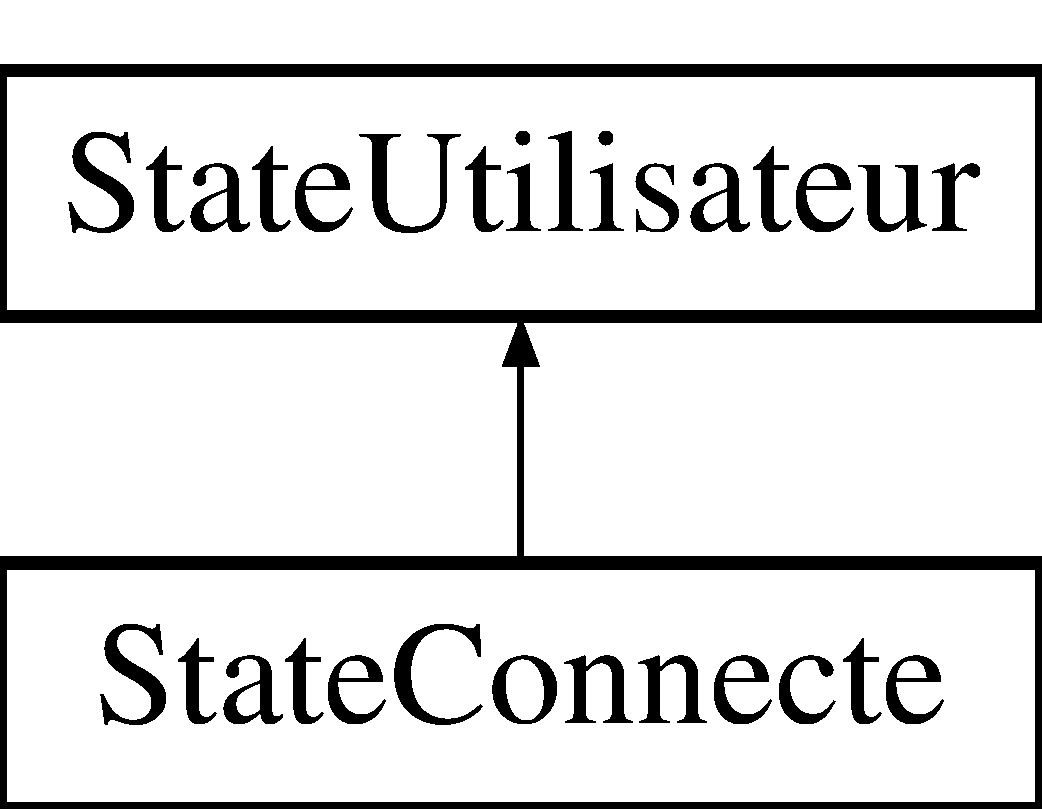
\includegraphics[height=2.000000cm]{classStateConnecte}
\end{center}
\end{figure}
\subsection*{Public Member Functions}
\begin{DoxyCompactItemize}
\item 
\hyperlink{classStateConnecte_a50922448c2191a173fae252dc32bc249}{State\-Connecte} (\hyperlink{classUtilisateur}{Utilisateur} $\ast$cont)
\begin{DoxyCompactList}\small\item\em Crée une instance d'état connecté pour l'\hyperlink{classUtilisateur}{Utilisateur} cont. \end{DoxyCompactList}\item 
\hypertarget{classStateConnecte_a2d03971c5edf05616d2faa5afba90925}{virtual void \hyperlink{classStateConnecte_a2d03971c5edf05616d2faa5afba90925}{deconnexion} ()}\label{classStateConnecte_a2d03971c5edf05616d2faa5afba90925}

\begin{DoxyCompactList}\small\item\em Permet de déconnecter un \hyperlink{classUtilisateur}{Utilisateur} connecté \end{DoxyCompactList}\item 
virtual std\-::string \hyperlink{classStateConnecte_aba8d7baa6105179fc820488532ee6914}{get\-Nom\-Etat} () const 
\begin{DoxyCompactList}\small\item\em Récupère le nom de l'état actuel de l'\hyperlink{classUtilisateur}{Utilisateur}. \end{DoxyCompactList}\item 
virtual void \hyperlink{classStateConnecte_a2c51f0790e9def5f4dcce2195af6c550}{vendre\-Produit} (int i, std\-::string nom, int prix, int quantite, bool enchere)
\begin{DoxyCompactList}\small\item\em Permet à un \hyperlink{classUtilisateur}{Utilisateur} connecté de vendre un \hyperlink{classProduit}{Produit}. \end{DoxyCompactList}\item 
\hypertarget{classStateConnecte_ab23a2c01a9e9a8116fa0add4a10cc798}{virtual void \hyperlink{classStateConnecte_ab23a2c01a9e9a8116fa0add4a10cc798}{acheter\-Produit} (int id, int quantite)}\label{classStateConnecte_ab23a2c01a9e9a8116fa0add4a10cc798}

\begin{DoxyCompactList}\small\item\em Permet à un \hyperlink{classUtilisateur}{Utilisateur} connecté d'acheter un \hyperlink{classProduit}{Produit} id. \end{DoxyCompactList}\item 
\hypertarget{classStateConnecte_a089f92126a87eaab2d4f070a9cdbdab9}{virtual void \hyperlink{classStateConnecte_a089f92126a87eaab2d4f070a9cdbdab9}{encherir} (int id, int prix)}\label{classStateConnecte_a089f92126a87eaab2d4f070a9cdbdab9}

\begin{DoxyCompactList}\small\item\em Permet à un \hyperlink{classUtilisateur}{Utilisateur} connecté d'enchérir sur un \hyperlink{classProduit}{Produit} id. \end{DoxyCompactList}\end{DoxyCompactItemize}
\subsection*{Additional Inherited Members}


\subsection{Detailed Description}
Classe concrète de l'état connecté des Utilisateurs. 

\subsection{Constructor \& Destructor Documentation}
\hypertarget{classStateConnecte_a50922448c2191a173fae252dc32bc249}{\index{State\-Connecte@{State\-Connecte}!State\-Connecte@{State\-Connecte}}
\index{State\-Connecte@{State\-Connecte}!StateConnecte@{State\-Connecte}}
\subsubsection[{State\-Connecte}]{\setlength{\rightskip}{0pt plus 5cm}State\-Connecte\-::\-State\-Connecte (
\begin{DoxyParamCaption}
\item[{{\bf Utilisateur} $\ast$}]{cont}
\end{DoxyParamCaption}
)\hspace{0.3cm}{\ttfamily [inline]}}}\label{classStateConnecte_a50922448c2191a173fae252dc32bc249}


Crée une instance d'état connecté pour l'\hyperlink{classUtilisateur}{Utilisateur} cont. 


\begin{DoxyParams}{Parameters}
{\em cont} & \-: un pointeur sur un \hyperlink{classUtilisateur}{Utilisateur} \\
\hline
\end{DoxyParams}


\subsection{Member Function Documentation}
\hypertarget{classStateConnecte_aba8d7baa6105179fc820488532ee6914}{\index{State\-Connecte@{State\-Connecte}!get\-Nom\-Etat@{get\-Nom\-Etat}}
\index{get\-Nom\-Etat@{get\-Nom\-Etat}!StateConnecte@{State\-Connecte}}
\subsubsection[{get\-Nom\-Etat}]{\setlength{\rightskip}{0pt plus 5cm}virtual std\-::string State\-Connecte\-::get\-Nom\-Etat (
\begin{DoxyParamCaption}
{}
\end{DoxyParamCaption}
) const\hspace{0.3cm}{\ttfamily [virtual]}}}\label{classStateConnecte_aba8d7baa6105179fc820488532ee6914}


Récupère le nom de l'état actuel de l'\hyperlink{classUtilisateur}{Utilisateur}. 

\begin{DoxyReturn}{Returns}
Un string contenant l'état 
\end{DoxyReturn}


Implements \hyperlink{classStateUtilisateur_aa0905985b352d22fd18ecbfae5d319a8}{State\-Utilisateur}.

\hypertarget{classStateConnecte_a2c51f0790e9def5f4dcce2195af6c550}{\index{State\-Connecte@{State\-Connecte}!vendre\-Produit@{vendre\-Produit}}
\index{vendre\-Produit@{vendre\-Produit}!StateConnecte@{State\-Connecte}}
\subsubsection[{vendre\-Produit}]{\setlength{\rightskip}{0pt plus 5cm}virtual void State\-Connecte\-::vendre\-Produit (
\begin{DoxyParamCaption}
\item[{int}]{i, }
\item[{std\-::string}]{nom, }
\item[{int}]{prix, }
\item[{int}]{quantite, }
\item[{bool}]{enchere}
\end{DoxyParamCaption}
)\hspace{0.3cm}{\ttfamily [virtual]}}}\label{classStateConnecte_a2c51f0790e9def5f4dcce2195af6c550}


Permet à un \hyperlink{classUtilisateur}{Utilisateur} connecté de vendre un \hyperlink{classProduit}{Produit}. 


\begin{DoxyParams}{Parameters}
{\em Les} & infos du \hyperlink{classProduit}{Produit} \\
\hline
\end{DoxyParams}


Reimplemented from \hyperlink{classStateUtilisateur_aa039ece92cb1663b9badf6ce4926fe1c}{State\-Utilisateur}.



The documentation for this class was generated from the following file\-:\begin{DoxyCompactItemize}
\item 
include/State\-Connecte.\-hpp\end{DoxyCompactItemize}

\hypertarget{classStateDeconnecte}{\section{State\-Deconnecte Class Reference}
\label{classStateDeconnecte}\index{State\-Deconnecte@{State\-Deconnecte}}
}


Classe concrète de l'état déconnecté des Utilisateurs.  




{\ttfamily \#include $<$State\-Deconnecte.\-hpp$>$}

Inheritance diagram for State\-Deconnecte\-:\begin{figure}[H]
\begin{center}
\leavevmode
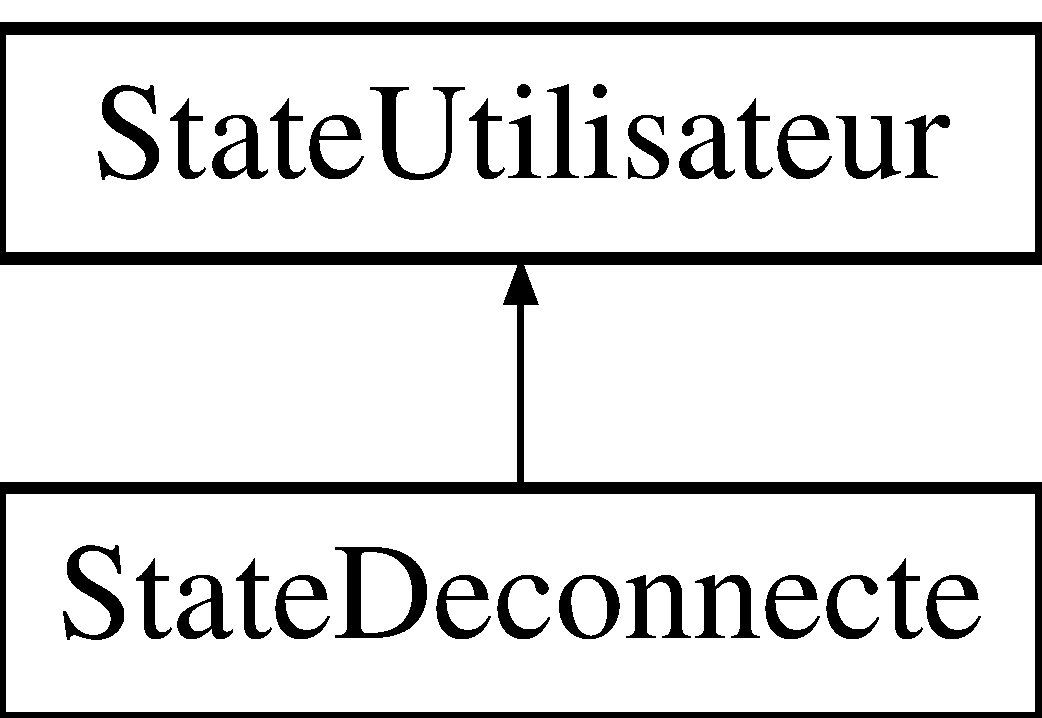
\includegraphics[height=2.000000cm]{classStateDeconnecte}
\end{center}
\end{figure}
\subsection*{Public Member Functions}
\begin{DoxyCompactItemize}
\item 
\hyperlink{classStateDeconnecte_a2f4fe61f40b06f055911b92e6a8a7ee8}{State\-Deconnecte} (\hyperlink{classUtilisateur}{Utilisateur} $\ast$cont)
\begin{DoxyCompactList}\small\item\em Crée une instance d'état déconnecté pour l'\hyperlink{classUtilisateur}{Utilisateur} cont. \end{DoxyCompactList}\item 
virtual void \hyperlink{classStateDeconnecte_af7a2a59f8b4fb3abe585a013cefa360a}{connexion} (std\-::string nom\-Util, std\-::string mdp)
\begin{DoxyCompactList}\small\item\em Permet de connecter un \hyperlink{classUtilisateur}{Utilisateur} déconnecté \end{DoxyCompactList}\item 
virtual void \hyperlink{classStateDeconnecte_a310df467d4d531402ee11b1d8469d1b6}{creer\-Compte} (std\-::string $\ast$infos)
\begin{DoxyCompactList}\small\item\em Permet de set les infos de l'\hyperlink{classUtilisateur}{Utilisateur}. \end{DoxyCompactList}\item 
virtual std\-::string \hyperlink{classStateDeconnecte_ac343c36edc1c66cf4b06b50b8b874654}{get\-Nom\-Etat} () const 
\begin{DoxyCompactList}\small\item\em Récupère le nom de l'état actuel de l'\hyperlink{classUtilisateur}{Utilisateur}. \end{DoxyCompactList}\end{DoxyCompactItemize}
\subsection*{Additional Inherited Members}


\subsection{Detailed Description}
Classe concrète de l'état déconnecté des Utilisateurs. 

\subsection{Constructor \& Destructor Documentation}
\hypertarget{classStateDeconnecte_a2f4fe61f40b06f055911b92e6a8a7ee8}{\index{State\-Deconnecte@{State\-Deconnecte}!State\-Deconnecte@{State\-Deconnecte}}
\index{State\-Deconnecte@{State\-Deconnecte}!StateDeconnecte@{State\-Deconnecte}}
\subsubsection[{State\-Deconnecte}]{\setlength{\rightskip}{0pt plus 5cm}State\-Deconnecte\-::\-State\-Deconnecte (
\begin{DoxyParamCaption}
\item[{{\bf Utilisateur} $\ast$}]{cont}
\end{DoxyParamCaption}
)}}\label{classStateDeconnecte_a2f4fe61f40b06f055911b92e6a8a7ee8}


Crée une instance d'état déconnecté pour l'\hyperlink{classUtilisateur}{Utilisateur} cont. 


\begin{DoxyParams}{Parameters}
{\em cont} & \-: un pointeur sur un \hyperlink{classUtilisateur}{Utilisateur} \\
\hline
\end{DoxyParams}


\subsection{Member Function Documentation}
\hypertarget{classStateDeconnecte_af7a2a59f8b4fb3abe585a013cefa360a}{\index{State\-Deconnecte@{State\-Deconnecte}!connexion@{connexion}}
\index{connexion@{connexion}!StateDeconnecte@{State\-Deconnecte}}
\subsubsection[{connexion}]{\setlength{\rightskip}{0pt plus 5cm}virtual void State\-Deconnecte\-::connexion (
\begin{DoxyParamCaption}
\item[{std\-::string}]{pseudo, }
\item[{std\-::string}]{mdp}
\end{DoxyParamCaption}
)\hspace{0.3cm}{\ttfamily [virtual]}}}\label{classStateDeconnecte_af7a2a59f8b4fb3abe585a013cefa360a}


Permet de connecter un \hyperlink{classUtilisateur}{Utilisateur} déconnecté 


\begin{DoxyParams}{Parameters}
{\em nom\-Util} & \-: nom d'utilisateur, pseudo ou mail ? \\
\hline
{\em mdp} & \-: mot de passe, en clair \\
\hline
\end{DoxyParams}


Reimplemented from \hyperlink{classStateUtilisateur_acf5e22c491f018f44114b4de2e22cba2}{State\-Utilisateur}.

\hypertarget{classStateDeconnecte_a310df467d4d531402ee11b1d8469d1b6}{\index{State\-Deconnecte@{State\-Deconnecte}!creer\-Compte@{creer\-Compte}}
\index{creer\-Compte@{creer\-Compte}!StateDeconnecte@{State\-Deconnecte}}
\subsubsection[{creer\-Compte}]{\setlength{\rightskip}{0pt plus 5cm}virtual void State\-Deconnecte\-::creer\-Compte (
\begin{DoxyParamCaption}
\item[{std\-::string $\ast$}]{infos}
\end{DoxyParamCaption}
)\hspace{0.3cm}{\ttfamily [virtual]}}}\label{classStateDeconnecte_a310df467d4d531402ee11b1d8469d1b6}


Permet de set les infos de l'\hyperlink{classUtilisateur}{Utilisateur}. 


\begin{DoxyParams}{Parameters}
{\em infos} & \-: un tableau de string contenant les infos du compte (nom, prénom, etc.) \\
\hline
\end{DoxyParams}


Reimplemented from \hyperlink{classStateUtilisateur_a46a74017e52db98001f089e67f4dd7d1}{State\-Utilisateur}.

\hypertarget{classStateDeconnecte_ac343c36edc1c66cf4b06b50b8b874654}{\index{State\-Deconnecte@{State\-Deconnecte}!get\-Nom\-Etat@{get\-Nom\-Etat}}
\index{get\-Nom\-Etat@{get\-Nom\-Etat}!StateDeconnecte@{State\-Deconnecte}}
\subsubsection[{get\-Nom\-Etat}]{\setlength{\rightskip}{0pt plus 5cm}virtual std\-::string State\-Deconnecte\-::get\-Nom\-Etat (
\begin{DoxyParamCaption}
{}
\end{DoxyParamCaption}
) const\hspace{0.3cm}{\ttfamily [virtual]}}}\label{classStateDeconnecte_ac343c36edc1c66cf4b06b50b8b874654}


Récupère le nom de l'état actuel de l'\hyperlink{classUtilisateur}{Utilisateur}. 

\begin{DoxyReturn}{Returns}
Un string contenant l'état 
\end{DoxyReturn}


Implements \hyperlink{classStateUtilisateur_aa0905985b352d22fd18ecbfae5d319a8}{State\-Utilisateur}.



The documentation for this class was generated from the following file\-:\begin{DoxyCompactItemize}
\item 
include/State\-Deconnecte.\-hpp\end{DoxyCompactItemize}

\hypertarget{classStateEnchere}{\section{State\-Enchere Class Reference}
\label{classStateEnchere}\index{State\-Enchere@{State\-Enchere}}
}


Classe concrète de l'état d'un \hyperlink{classProduit}{Produit} mis aux enchères.  




{\ttfamily \#include $<$State\-Enchere.\-hpp$>$}

Inheritance diagram for State\-Enchere\-:\begin{figure}[H]
\begin{center}
\leavevmode
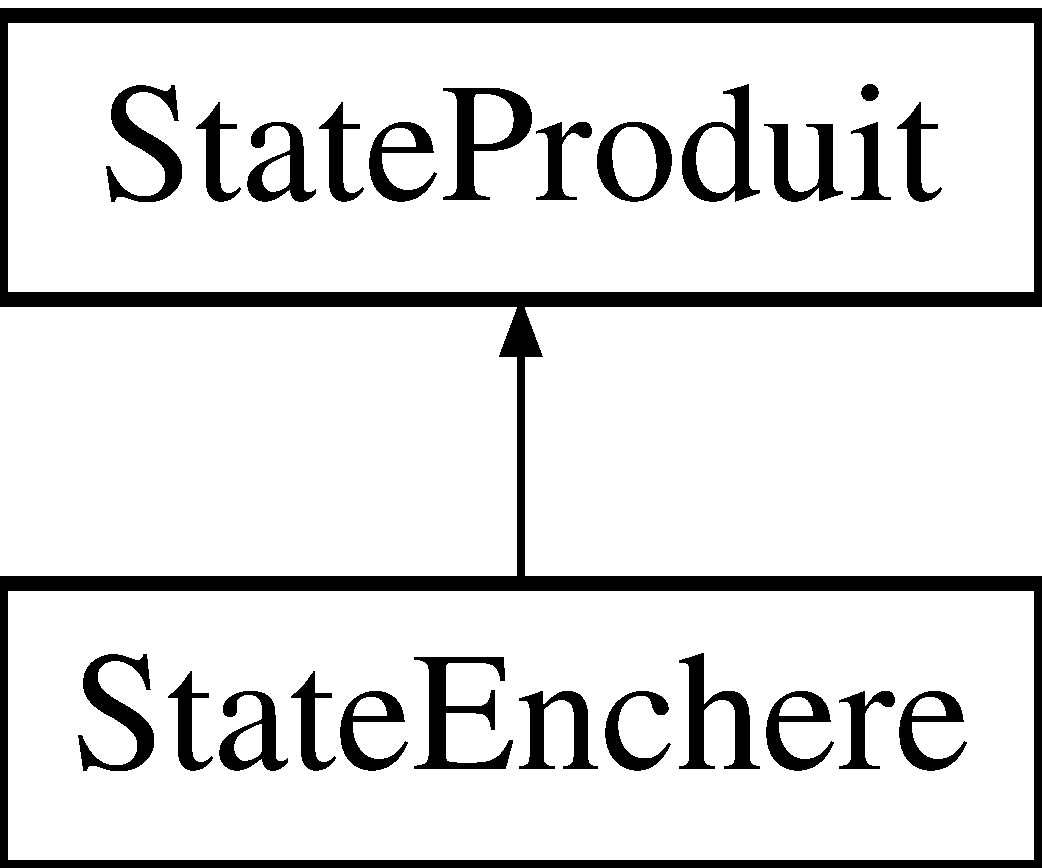
\includegraphics[height=2.000000cm]{classStateEnchere}
\end{center}
\end{figure}
\subsection*{Public Member Functions}
\begin{DoxyCompactItemize}
\item 
\hypertarget{classStateEnchere_a8038385efd919bfdf6a3da9c96c99368}{{\bfseries State\-Enchere} (\hyperlink{classProduit}{Produit} $\ast$cont)}\label{classStateEnchere_a8038385efd919bfdf6a3da9c96c99368}

\item 
virtual std\-::string \hyperlink{classStateEnchere_a2c6ccc2c404381333ed64488568d34aa}{get\-Nom\-Etat} () const 
\begin{DoxyCompactList}\small\item\em Permet de récupérer le nom d'un état. \end{DoxyCompactList}\end{DoxyCompactItemize}
\subsection*{Additional Inherited Members}


\subsection{Detailed Description}
Classe concrète de l'état d'un \hyperlink{classProduit}{Produit} mis aux enchères. 

\subsection{Member Function Documentation}
\hypertarget{classStateEnchere_a2c6ccc2c404381333ed64488568d34aa}{\index{State\-Enchere@{State\-Enchere}!get\-Nom\-Etat@{get\-Nom\-Etat}}
\index{get\-Nom\-Etat@{get\-Nom\-Etat}!StateEnchere@{State\-Enchere}}
\subsubsection[{get\-Nom\-Etat}]{\setlength{\rightskip}{0pt plus 5cm}virtual std\-::string State\-Enchere\-::get\-Nom\-Etat (
\begin{DoxyParamCaption}
{}
\end{DoxyParamCaption}
) const\hspace{0.3cm}{\ttfamily [virtual]}}}\label{classStateEnchere_a2c6ccc2c404381333ed64488568d34aa}


Permet de récupérer le nom d'un état. 


\begin{DoxyParams}{Parameters}
{\em } & le nom de l'état \\
\hline
\end{DoxyParams}


Implements \hyperlink{classStateProduit_aada1a1cc10d67e886b96322683c05411}{State\-Produit}.



The documentation for this class was generated from the following file\-:\begin{DoxyCompactItemize}
\item 
include/State\-Enchere.\-hpp\end{DoxyCompactItemize}

\hypertarget{classStateNormal}{\section{State\-Normal Class Reference}
\label{classStateNormal}\index{State\-Normal@{State\-Normal}}
}


Classe concrète de l'état d'un \hyperlink{classProduit}{Produit} mis en vente directe.  




{\ttfamily \#include $<$State\-Normal.\-hpp$>$}

Inheritance diagram for State\-Normal\-:\begin{figure}[H]
\begin{center}
\leavevmode
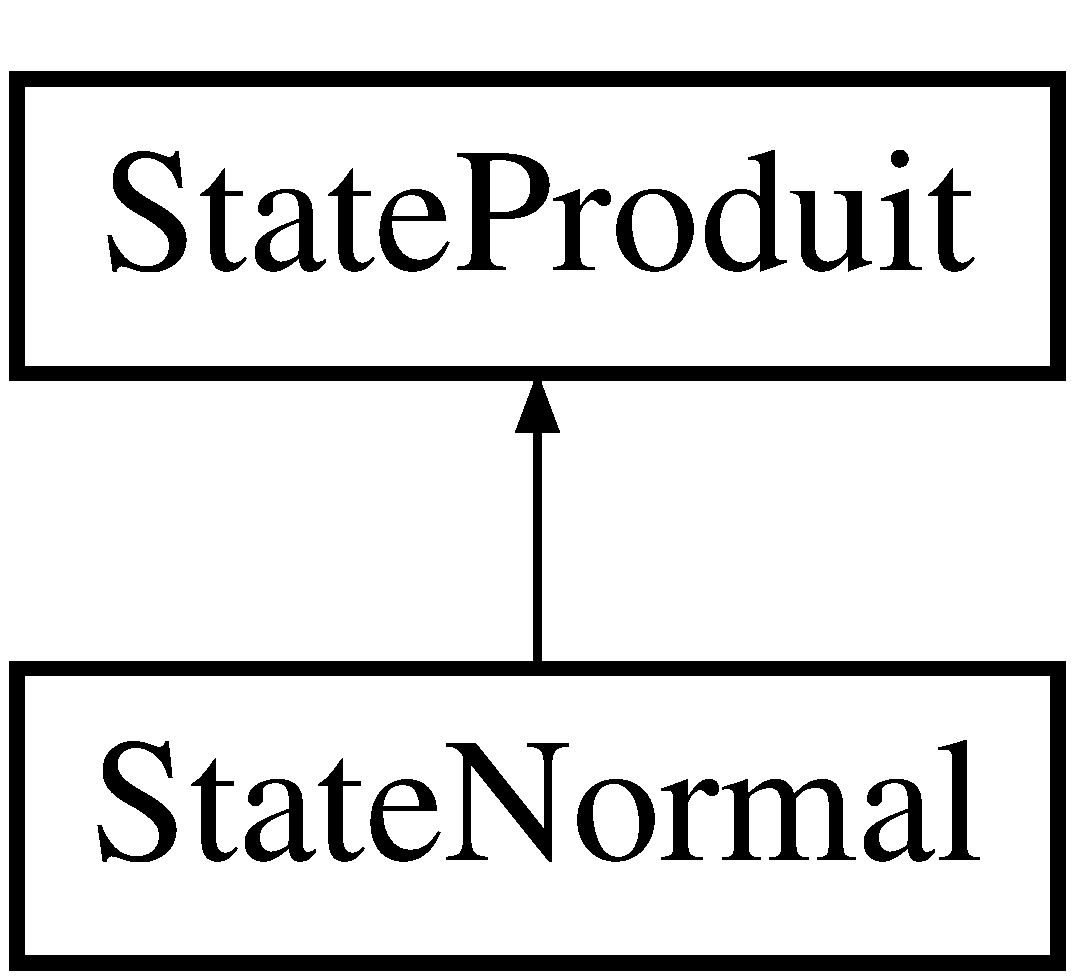
\includegraphics[height=2.000000cm]{classStateNormal}
\end{center}
\end{figure}
\subsection*{Public Member Functions}
\begin{DoxyCompactItemize}
\item 
\hypertarget{classStateNormal_a3002ec27b5e26a0bf106c02012fe3436}{{\bfseries State\-Normal} (\hyperlink{classProduit}{Produit} $\ast$cont)}\label{classStateNormal_a3002ec27b5e26a0bf106c02012fe3436}

\item 
virtual std\-::string \hyperlink{classStateNormal_a6e8a998e6c13aafdc49c11eb0907e1ec}{get\-Nom\-Etat} () const 
\begin{DoxyCompactList}\small\item\em Permet de récupérer le nom d'un état. \end{DoxyCompactList}\end{DoxyCompactItemize}
\subsection*{Additional Inherited Members}


\subsection{Detailed Description}
Classe concrète de l'état d'un \hyperlink{classProduit}{Produit} mis en vente directe. 

\subsection{Member Function Documentation}
\hypertarget{classStateNormal_a6e8a998e6c13aafdc49c11eb0907e1ec}{\index{State\-Normal@{State\-Normal}!get\-Nom\-Etat@{get\-Nom\-Etat}}
\index{get\-Nom\-Etat@{get\-Nom\-Etat}!StateNormal@{State\-Normal}}
\subsubsection[{get\-Nom\-Etat}]{\setlength{\rightskip}{0pt plus 5cm}virtual std\-::string State\-Normal\-::get\-Nom\-Etat (
\begin{DoxyParamCaption}
{}
\end{DoxyParamCaption}
) const\hspace{0.3cm}{\ttfamily [virtual]}}}\label{classStateNormal_a6e8a998e6c13aafdc49c11eb0907e1ec}


Permet de récupérer le nom d'un état. 


\begin{DoxyParams}{Parameters}
{\em } & le nom de l'état \\
\hline
\end{DoxyParams}


Implements \hyperlink{classStateProduit_aada1a1cc10d67e886b96322683c05411}{State\-Produit}.



The documentation for this class was generated from the following file\-:\begin{DoxyCompactItemize}
\item 
include/State\-Normal.\-hpp\end{DoxyCompactItemize}

\hypertarget{classStateProduit}{\section{State\-Produit Class Reference}
\label{classStateProduit}\index{State\-Produit@{State\-Produit}}
}


Classe abstraite qui sera héritée par les états concrets (Normal et Enchères) Dans notre implémentation, un \hyperlink{classProduit}{Produit} connait un Etat à la fois. Cet Etat connait lui aussi le \hyperlink{classProduit}{Produit}, passé en paramètre du constructeur, pour pouvoir appeler ses fonctions localement. L'état étant propre à une instance de \hyperlink{classProduit}{Produit}, c'est \hyperlink{classProduit}{Produit} qui se chargera de le détruire.  




{\ttfamily \#include $<$State\-Produit.\-hpp$>$}

Inheritance diagram for State\-Produit\-:\begin{figure}[H]
\begin{center}
\leavevmode
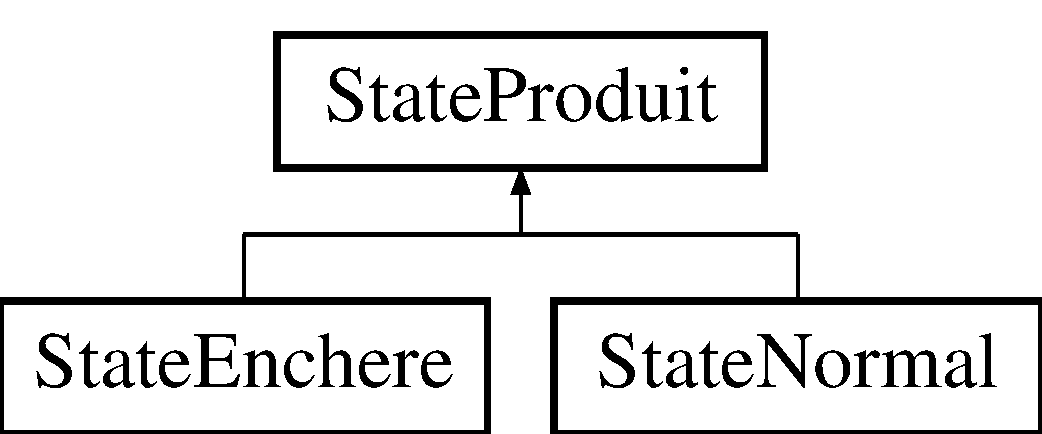
\includegraphics[height=2.000000cm]{classStateProduit}
\end{center}
\end{figure}
\subsection*{Public Member Functions}
\begin{DoxyCompactItemize}
\item 
virtual std\-::string \hyperlink{classStateProduit_aada1a1cc10d67e886b96322683c05411}{get\-Nom\-Etat} () const =0
\begin{DoxyCompactList}\small\item\em Permet de récupérer le nom d'un état. \end{DoxyCompactList}\end{DoxyCompactItemize}
\subsection*{Protected Member Functions}
\begin{DoxyCompactItemize}
\item 
\hyperlink{classStateProduit_ae79072739c68f66c8b39958a376b6c3f}{State\-Produit} (\hyperlink{classProduit}{Produit} $\ast$cont)
\begin{DoxyCompactList}\small\item\em Crée un état sur un \hyperlink{classProduit}{Produit}. \end{DoxyCompactList}\end{DoxyCompactItemize}
\subsection*{Protected Attributes}
\begin{DoxyCompactItemize}
\item 
\hypertarget{classStateProduit_acc1a34648aacca5b0646c5b7369e14ba}{\hyperlink{classProduit}{Produit} $\ast$ {\bfseries \-\_\-context}}\label{classStateProduit_acc1a34648aacca5b0646c5b7369e14ba}

\end{DoxyCompactItemize}


\subsection{Detailed Description}
Classe abstraite qui sera héritée par les états concrets (Normal et Enchères) Dans notre implémentation, un \hyperlink{classProduit}{Produit} connait un Etat à la fois. Cet Etat connait lui aussi le \hyperlink{classProduit}{Produit}, passé en paramètre du constructeur, pour pouvoir appeler ses fonctions localement. L'état étant propre à une instance de \hyperlink{classProduit}{Produit}, c'est \hyperlink{classProduit}{Produit} qui se chargera de le détruire. 

\subsection{Constructor \& Destructor Documentation}
\hypertarget{classStateProduit_ae79072739c68f66c8b39958a376b6c3f}{\index{State\-Produit@{State\-Produit}!State\-Produit@{State\-Produit}}
\index{State\-Produit@{State\-Produit}!StateProduit@{State\-Produit}}
\subsubsection[{State\-Produit}]{\setlength{\rightskip}{0pt plus 5cm}State\-Produit\-::\-State\-Produit (
\begin{DoxyParamCaption}
\item[{{\bf Produit} $\ast$}]{cont}
\end{DoxyParamCaption}
)\hspace{0.3cm}{\ttfamily [inline]}, {\ttfamily [protected]}}}\label{classStateProduit_ae79072739c68f66c8b39958a376b6c3f}


Crée un état sur un \hyperlink{classProduit}{Produit}. 

Pointeur sur le \hyperlink{classProduit}{Produit} qui sera associé à cet état
\begin{DoxyParams}{Parameters}
{\em cont} & \-: Un pointeur sur un état \\
\hline
\end{DoxyParams}


\subsection{Member Function Documentation}
\hypertarget{classStateProduit_aada1a1cc10d67e886b96322683c05411}{\index{State\-Produit@{State\-Produit}!get\-Nom\-Etat@{get\-Nom\-Etat}}
\index{get\-Nom\-Etat@{get\-Nom\-Etat}!StateProduit@{State\-Produit}}
\subsubsection[{get\-Nom\-Etat}]{\setlength{\rightskip}{0pt plus 5cm}virtual std\-::string State\-Produit\-::get\-Nom\-Etat (
\begin{DoxyParamCaption}
{}
\end{DoxyParamCaption}
) const\hspace{0.3cm}{\ttfamily [pure virtual]}}}\label{classStateProduit_aada1a1cc10d67e886b96322683c05411}


Permet de récupérer le nom d'un état. 


\begin{DoxyParams}{Parameters}
{\em } & le nom de l'état \\
\hline
\end{DoxyParams}


Implemented in \hyperlink{classStateEnchere_a2c6ccc2c404381333ed64488568d34aa}{State\-Enchere}, and \hyperlink{classStateNormal_a6e8a998e6c13aafdc49c11eb0907e1ec}{State\-Normal}.



The documentation for this class was generated from the following file\-:\begin{DoxyCompactItemize}
\item 
include/State\-Produit.\-hpp\end{DoxyCompactItemize}

\hypertarget{classStateUtilisateur}{\section{State\-Utilisateur Class Reference}
\label{classStateUtilisateur}\index{State\-Utilisateur@{State\-Utilisateur}}
}


Classe abstraite qui sera héritée par les états concrets (Connecté et Déconnecté) Dans notre implémentation, un \hyperlink{classUtilisateur}{Utilisateur} connait un Etat à la fois. Cet Etat connait lui aussi l'\hyperlink{classUtilisateur}{Utilisateur}, passé en paramètre du constructeur, pour pouvoir appeler ses fonctions localement. Quand l'état actuel va appeler une fonction de changement d'état (connexion ou déconnexion), il va set un nouvel état à l'\hyperlink{classUtilisateur}{Utilisateur} avant de se supprimer.  




{\ttfamily \#include $<$State\-Utilisateur.\-hpp$>$}

Inheritance diagram for State\-Utilisateur\-:\begin{figure}[H]
\begin{center}
\leavevmode
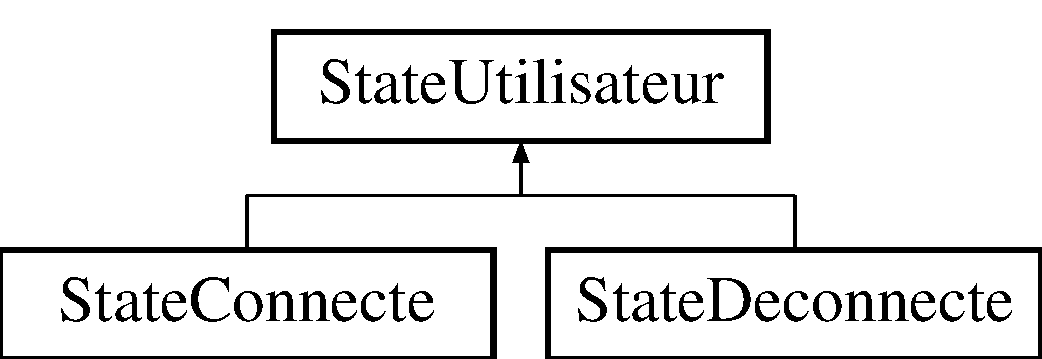
\includegraphics[height=2.000000cm]{classStateUtilisateur}
\end{center}
\end{figure}
\subsection*{Public Member Functions}
\begin{DoxyCompactItemize}
\item 
virtual void \hyperlink{classStateUtilisateur_acf5e22c491f018f44114b4de2e22cba2}{connexion} (std\-::string pseudo, std\-::string mdp)
\begin{DoxyCompactList}\small\item\em Permet de connecter un \hyperlink{classUtilisateur}{Utilisateur} déconnecté \end{DoxyCompactList}\item 
\hypertarget{classStateUtilisateur_a7219631d1a792b86e6cb1baaed036cdd}{virtual void \hyperlink{classStateUtilisateur_a7219631d1a792b86e6cb1baaed036cdd}{deconnexion} ()}\label{classStateUtilisateur_a7219631d1a792b86e6cb1baaed036cdd}

\begin{DoxyCompactList}\small\item\em Permet de déconnecter un \hyperlink{classUtilisateur}{Utilisateur} connecté \end{DoxyCompactList}\item 
virtual void \hyperlink{classStateUtilisateur_a46a74017e52db98001f089e67f4dd7d1}{creer\-Compte} (std\-::string $\ast$infos)
\begin{DoxyCompactList}\small\item\em Permet de set les infos de l'\hyperlink{classUtilisateur}{Utilisateur}. \end{DoxyCompactList}\item 
virtual std\-::string \hyperlink{classStateUtilisateur_aa0905985b352d22fd18ecbfae5d319a8}{get\-Nom\-Etat} () const =0
\begin{DoxyCompactList}\small\item\em Récupère le nom de l'état actuel de l'\hyperlink{classUtilisateur}{Utilisateur}. \end{DoxyCompactList}\item 
\hypertarget{classStateUtilisateur_a6312084252e725b07f3061aed8530eae}{virtual void \hyperlink{classStateUtilisateur_a6312084252e725b07f3061aed8530eae}{acheter\-Produit} (int id, int quantite)}\label{classStateUtilisateur_a6312084252e725b07f3061aed8530eae}

\begin{DoxyCompactList}\small\item\em Permet à un \hyperlink{classUtilisateur}{Utilisateur} connecté d'acheter un \hyperlink{classProduit}{Produit} id. \end{DoxyCompactList}\item 
\hypertarget{classStateUtilisateur_a4e20c37e50a369d6f1263776992ada7c}{virtual void \hyperlink{classStateUtilisateur_a4e20c37e50a369d6f1263776992ada7c}{encherir} (int id, int prix)}\label{classStateUtilisateur_a4e20c37e50a369d6f1263776992ada7c}

\begin{DoxyCompactList}\small\item\em Permet à un \hyperlink{classUtilisateur}{Utilisateur} connecté d'enchérir sur un \hyperlink{classProduit}{Produit} id. \end{DoxyCompactList}\item 
virtual void \hyperlink{classStateUtilisateur_aa039ece92cb1663b9badf6ce4926fe1c}{vendre\-Produit} (int i, std\-::string nom, int prix, int quantite, bool enchere)
\begin{DoxyCompactList}\small\item\em Permet à un \hyperlink{classUtilisateur}{Utilisateur} connecté de vendre un \hyperlink{classProduit}{Produit}. \end{DoxyCompactList}\end{DoxyCompactItemize}
\subsection*{Protected Member Functions}
\begin{DoxyCompactItemize}
\item 
\hyperlink{classStateUtilisateur_a336272db2eba31466abb07ae866f55d4}{State\-Utilisateur} (\hyperlink{classUtilisateur}{Utilisateur} $\ast$cont)
\end{DoxyCompactItemize}
\subsection*{Protected Attributes}
\begin{DoxyCompactItemize}
\item 
\hypertarget{classStateUtilisateur_a7ba23f1ccfadd18e04bdc2ab2653b845}{\hyperlink{classUtilisateur}{Utilisateur} $\ast$ {\bfseries \-\_\-context}}\label{classStateUtilisateur_a7ba23f1ccfadd18e04bdc2ab2653b845}

\end{DoxyCompactItemize}


\subsection{Detailed Description}
Classe abstraite qui sera héritée par les états concrets (Connecté et Déconnecté) Dans notre implémentation, un \hyperlink{classUtilisateur}{Utilisateur} connait un Etat à la fois. Cet Etat connait lui aussi l'\hyperlink{classUtilisateur}{Utilisateur}, passé en paramètre du constructeur, pour pouvoir appeler ses fonctions localement. Quand l'état actuel va appeler une fonction de changement d'état (connexion ou déconnexion), il va set un nouvel état à l'\hyperlink{classUtilisateur}{Utilisateur} avant de se supprimer. 

\subsection{Constructor \& Destructor Documentation}
\hypertarget{classStateUtilisateur_a336272db2eba31466abb07ae866f55d4}{\index{State\-Utilisateur@{State\-Utilisateur}!State\-Utilisateur@{State\-Utilisateur}}
\index{State\-Utilisateur@{State\-Utilisateur}!StateUtilisateur@{State\-Utilisateur}}
\subsubsection[{State\-Utilisateur}]{\setlength{\rightskip}{0pt plus 5cm}State\-Utilisateur\-::\-State\-Utilisateur (
\begin{DoxyParamCaption}
\item[{{\bf Utilisateur} $\ast$}]{cont}
\end{DoxyParamCaption}
)\hspace{0.3cm}{\ttfamily [inline]}, {\ttfamily [protected]}}}\label{classStateUtilisateur_a336272db2eba31466abb07ae866f55d4}
L'\hyperlink{classUtilisateur}{Utilisateur} lié à cet état 
\begin{DoxyParams}{Parameters}
{\em cont} & \-: Un pointeur sur un \hyperlink{classUtilisateur}{Utilisateur} \\
\hline
\end{DoxyParams}


\subsection{Member Function Documentation}
\hypertarget{classStateUtilisateur_acf5e22c491f018f44114b4de2e22cba2}{\index{State\-Utilisateur@{State\-Utilisateur}!connexion@{connexion}}
\index{connexion@{connexion}!StateUtilisateur@{State\-Utilisateur}}
\subsubsection[{connexion}]{\setlength{\rightskip}{0pt plus 5cm}virtual void State\-Utilisateur\-::connexion (
\begin{DoxyParamCaption}
\item[{std\-::string}]{pseudo, }
\item[{std\-::string}]{mdp}
\end{DoxyParamCaption}
)\hspace{0.3cm}{\ttfamily [virtual]}}}\label{classStateUtilisateur_acf5e22c491f018f44114b4de2e22cba2}


Permet de connecter un \hyperlink{classUtilisateur}{Utilisateur} déconnecté 


\begin{DoxyParams}{Parameters}
{\em nom\-Util} & \-: nom d'utilisateur, pseudo ou mail ? \\
\hline
{\em mdp} & \-: mot de passe, en clair \\
\hline
\end{DoxyParams}


Reimplemented in \hyperlink{classStateDeconnecte_af7a2a59f8b4fb3abe585a013cefa360a}{State\-Deconnecte}.

\hypertarget{classStateUtilisateur_a46a74017e52db98001f089e67f4dd7d1}{\index{State\-Utilisateur@{State\-Utilisateur}!creer\-Compte@{creer\-Compte}}
\index{creer\-Compte@{creer\-Compte}!StateUtilisateur@{State\-Utilisateur}}
\subsubsection[{creer\-Compte}]{\setlength{\rightskip}{0pt plus 5cm}virtual void State\-Utilisateur\-::creer\-Compte (
\begin{DoxyParamCaption}
\item[{std\-::string $\ast$}]{infos}
\end{DoxyParamCaption}
)\hspace{0.3cm}{\ttfamily [virtual]}}}\label{classStateUtilisateur_a46a74017e52db98001f089e67f4dd7d1}


Permet de set les infos de l'\hyperlink{classUtilisateur}{Utilisateur}. 


\begin{DoxyParams}{Parameters}
{\em infos} & \-: un tableau de string contenant les infos du compte (nom, prénom, etc.) \\
\hline
\end{DoxyParams}


Reimplemented in \hyperlink{classStateDeconnecte_a310df467d4d531402ee11b1d8469d1b6}{State\-Deconnecte}.

\hypertarget{classStateUtilisateur_aa0905985b352d22fd18ecbfae5d319a8}{\index{State\-Utilisateur@{State\-Utilisateur}!get\-Nom\-Etat@{get\-Nom\-Etat}}
\index{get\-Nom\-Etat@{get\-Nom\-Etat}!StateUtilisateur@{State\-Utilisateur}}
\subsubsection[{get\-Nom\-Etat}]{\setlength{\rightskip}{0pt plus 5cm}virtual std\-::string State\-Utilisateur\-::get\-Nom\-Etat (
\begin{DoxyParamCaption}
{}
\end{DoxyParamCaption}
) const\hspace{0.3cm}{\ttfamily [pure virtual]}}}\label{classStateUtilisateur_aa0905985b352d22fd18ecbfae5d319a8}


Récupère le nom de l'état actuel de l'\hyperlink{classUtilisateur}{Utilisateur}. 

\begin{DoxyReturn}{Returns}
Un string contenant l'état 
\end{DoxyReturn}


Implemented in \hyperlink{classStateDeconnecte_ac343c36edc1c66cf4b06b50b8b874654}{State\-Deconnecte}, and \hyperlink{classStateConnecte_aba8d7baa6105179fc820488532ee6914}{State\-Connecte}.

\hypertarget{classStateUtilisateur_aa039ece92cb1663b9badf6ce4926fe1c}{\index{State\-Utilisateur@{State\-Utilisateur}!vendre\-Produit@{vendre\-Produit}}
\index{vendre\-Produit@{vendre\-Produit}!StateUtilisateur@{State\-Utilisateur}}
\subsubsection[{vendre\-Produit}]{\setlength{\rightskip}{0pt plus 5cm}virtual void State\-Utilisateur\-::vendre\-Produit (
\begin{DoxyParamCaption}
\item[{int}]{i, }
\item[{std\-::string}]{nom, }
\item[{int}]{prix, }
\item[{int}]{quantite, }
\item[{bool}]{enchere}
\end{DoxyParamCaption}
)\hspace{0.3cm}{\ttfamily [virtual]}}}\label{classStateUtilisateur_aa039ece92cb1663b9badf6ce4926fe1c}


Permet à un \hyperlink{classUtilisateur}{Utilisateur} connecté de vendre un \hyperlink{classProduit}{Produit}. 


\begin{DoxyParams}{Parameters}
{\em Les} & infos du \hyperlink{classProduit}{Produit} \\
\hline
\end{DoxyParams}


Reimplemented in \hyperlink{classStateConnecte_a2c51f0790e9def5f4dcce2195af6c550}{State\-Connecte}.



The documentation for this class was generated from the following file\-:\begin{DoxyCompactItemize}
\item 
include/State\-Utilisateur.\-hpp\end{DoxyCompactItemize}

\hypertarget{classUtilisateur}{\section{Utilisateur Class Reference}
\label{classUtilisateur}\index{Utilisateur@{Utilisateur}}
}


Classe \hyperlink{classUtilisateur}{Utilisateur}, gérant toutes les données et les appels aux fonctions de son état. On stockera des instances de cette classe dans la bdd.  




{\ttfamily \#include $<$Utilisateur.\-hpp$>$}

\subsection*{Public Member Functions}
\begin{DoxyCompactItemize}
\item 
\hyperlink{classUtilisateur_ae76433a6d353c5f5ad0c6a6af64022ad}{Utilisateur} ()
\item 
\hyperlink{classUtilisateur_af766969b6d93c1e1dfda7d887fbf067d}{Utilisateur} (const \hyperlink{classUtilisateur}{Utilisateur} \&au)
\item 
\hyperlink{classUtilisateur_a6631539ceecd6140fe525eb91485537b}{$\sim$\-Utilisateur} ()
\item 
\hypertarget{classUtilisateur_a52c851867029c05a86b88853e00728e5}{std\-::string {\bfseries get\-Nom} () const }\label{classUtilisateur_a52c851867029c05a86b88853e00728e5}

\item 
\hypertarget{classUtilisateur_acfc6e7e8bfedf7456f74f9fba388fbe6}{std\-::string {\bfseries get\-Prenom} () const }\label{classUtilisateur_acfc6e7e8bfedf7456f74f9fba388fbe6}

\item 
\hypertarget{classUtilisateur_aaadcbac2ce02ef4bf9e060cc4cfadcc4}{std\-::string {\bfseries get\-Pseudo} () const }\label{classUtilisateur_aaadcbac2ce02ef4bf9e060cc4cfadcc4}

\item 
\hypertarget{classUtilisateur_a86643f2169c336c651612c11bf1b5a1e}{std\-::string {\bfseries get\-Mail} () const }\label{classUtilisateur_a86643f2169c336c651612c11bf1b5a1e}

\item 
\hypertarget{classUtilisateur_a74f21491b1263a248a8bae866d7386f2}{std\-::string {\bfseries get\-Mot\-De\-Passe} () const }\label{classUtilisateur_a74f21491b1263a248a8bae866d7386f2}

\item 
\hypertarget{classUtilisateur_a7756213c6af661d8e706e2295f0b8675}{std\-::string {\bfseries get\-Adresse\-Num} () const }\label{classUtilisateur_a7756213c6af661d8e706e2295f0b8675}

\item 
\hypertarget{classUtilisateur_a9869999edde2e38fb84aa731a60e2a4f}{std\-::string {\bfseries get\-Adresse\-C\-P} () const }\label{classUtilisateur_a9869999edde2e38fb84aa731a60e2a4f}

\item 
\hypertarget{classUtilisateur_ac61cba367187cb88c9d6d170ec7f9bad}{std\-::string {\bfseries get\-Adresse\-Ville} () const }\label{classUtilisateur_ac61cba367187cb88c9d6d170ec7f9bad}

\item 
\hypertarget{classUtilisateur_a5a79bcadd84048cd84e227308b51ae01}{std\-::string {\bfseries get\-Numero} () const }\label{classUtilisateur_a5a79bcadd84048cd84e227308b51ae01}

\item 
\hypertarget{classUtilisateur_a3f2d52048f66f37a0caaf4d1872664a2}{\hyperlink{classStateUtilisateur}{State\-Utilisateur} $\ast$ {\bfseries get\-Etat} ()}\label{classUtilisateur_a3f2d52048f66f37a0caaf4d1872664a2}

\item 
\hypertarget{classUtilisateur_ae64c47038e5786dfb003e755b1e1f432}{std\-::vector$<$ int $>$ {\bfseries get\-Histo\-Achat} () const }\label{classUtilisateur_ae64c47038e5786dfb003e755b1e1f432}

\item 
\hypertarget{classUtilisateur_a3c8c96807432b68f5f2aa0f4e01e8ce1}{std\-::vector$<$ int $>$ {\bfseries get\-Histo\-Vente} () const }\label{classUtilisateur_a3c8c96807432b68f5f2aa0f4e01e8ce1}

\item 
\hypertarget{classUtilisateur_a85dc60f77b270d74b7fa33147804575a}{\hyperlink{classBdd}{Bdd} $\ast$ {\bfseries get\-Bdd} () const }\label{classUtilisateur_a85dc60f77b270d74b7fa33147804575a}

\item 
\hyperlink{classProduit}{Produit} $\ast$ \hyperlink{classUtilisateur_aa62e585189589dc77a7edaf5afb3b7e4}{get\-Produit} (int id)
\begin{DoxyCompactList}\small\item\em Utilisée à des fin de réduction de couplage. \end{DoxyCompactList}\item 
\hypertarget{classUtilisateur_ae087f4d94434085de46f7b4698f2ee1f}{\hyperlink{classUtilisateur}{Utilisateur} $\ast$ {\bfseries get\-Utilisateur} (std\-::string nom\-Util, std\-::string mdp)}\label{classUtilisateur_ae087f4d94434085de46f7b4698f2ee1f}

\item 
\hypertarget{classUtilisateur_a17f8432b3d5e6e6fafb839926a16d1d8}{void {\bfseries set\-Bdd} (\hyperlink{classBdd}{Bdd} $\ast$b)}\label{classUtilisateur_a17f8432b3d5e6e6fafb839926a16d1d8}

\item 
\hypertarget{classUtilisateur_a22ffb78a049164a0a6f43e552d2cc933}{void {\bfseries set\-Etat} (\hyperlink{classStateUtilisateur}{State\-Utilisateur} $\ast$s)}\label{classUtilisateur_a22ffb78a049164a0a6f43e552d2cc933}

\item 
\hypertarget{classUtilisateur_a20a32b47f2b080a4aead49e16bd06f44}{void {\bfseries set\-Nom} (std\-::string n)}\label{classUtilisateur_a20a32b47f2b080a4aead49e16bd06f44}

\item 
\hypertarget{classUtilisateur_a82c09ccdcb2449ee5a9938bb716938b6}{void {\bfseries set\-Prenom} (std\-::string p)}\label{classUtilisateur_a82c09ccdcb2449ee5a9938bb716938b6}

\item 
\hypertarget{classUtilisateur_a8463c077b33ccc93c8e424a47b9bc369}{void {\bfseries set\-Pseudo} (std\-::string p)}\label{classUtilisateur_a8463c077b33ccc93c8e424a47b9bc369}

\item 
\hypertarget{classUtilisateur_a895f56e8a99f17da4953be6c790376aa}{void {\bfseries set\-Mail} (std\-::string m)}\label{classUtilisateur_a895f56e8a99f17da4953be6c790376aa}

\item 
\hypertarget{classUtilisateur_acb7689c9ca689a7915db6ddb163059ff}{void {\bfseries set\-Mot\-De\-Passe} (std\-::string mdp)}\label{classUtilisateur_acb7689c9ca689a7915db6ddb163059ff}

\item 
\hypertarget{classUtilisateur_aac03cf860595ffdac27ff2083f9ad28a}{void {\bfseries set\-Adresse\-Num} (std\-::string an)}\label{classUtilisateur_aac03cf860595ffdac27ff2083f9ad28a}

\item 
\hypertarget{classUtilisateur_a1ba2bb63014f22021c5de1d171658a57}{void {\bfseries set\-Adresse\-C\-P} (std\-::string acp)}\label{classUtilisateur_a1ba2bb63014f22021c5de1d171658a57}

\item 
\hypertarget{classUtilisateur_a70e72c792ef91b0007d6bfa8736a20b3}{void {\bfseries set\-Adresse\-Ville} (std\-::string av)}\label{classUtilisateur_a70e72c792ef91b0007d6bfa8736a20b3}

\item 
\hypertarget{classUtilisateur_a540cd06e80e20d97eda548ad25670c79}{void {\bfseries set\-Numero} (std\-::string n)}\label{classUtilisateur_a540cd06e80e20d97eda548ad25670c79}

\item 
void \hyperlink{classUtilisateur_a5e2d22fa977ec78efaeff34ba404878c}{add\-Histo\-Achat} (int id)
\begin{DoxyCompactList}\small\item\em Ajoute un produit dans l'historique d'achat de l'utilisateur. \end{DoxyCompactList}\item 
void \hyperlink{classUtilisateur_a23adc8461a76f9816dac9f87f2adb135}{add\-Histo\-Vente} (int id)
\begin{DoxyCompactList}\small\item\em Ajoute un produit dans l'historique de vente de l'utilisateur. \end{DoxyCompactList}\item 
void \hyperlink{classUtilisateur_ac586ef4afa8c85f56cca3c688732bb81}{creer\-Compte} (std\-::string $\ast$infos)
\begin{DoxyCompactList}\small\item\em Crée un compte et l'ajoute à la bdd. \end{DoxyCompactList}\item 
\hypertarget{classUtilisateur_ac10b85517b5b34b1357744a495537165}{void \hyperlink{classUtilisateur_ac10b85517b5b34b1357744a495537165}{vider} ()}\label{classUtilisateur_ac10b85517b5b34b1357744a495537165}

\begin{DoxyCompactList}\small\item\em Vide les champs de l'utilisateur (Peut être utilisé pour décrire un utilisateur déconnecté) \end{DoxyCompactList}\item 
void \hyperlink{classUtilisateur_a41b0d5ff30d82c9f68110fb6687f449a}{connexion} (std\-::string pseudo, std\-::string mdp)
\begin{DoxyCompactList}\small\item\em Définit l'utilisateur comme connecté \end{DoxyCompactList}\item 
\hypertarget{classUtilisateur_aed5a9ebdb82025692fa06622d9239cf7}{void \hyperlink{classUtilisateur_aed5a9ebdb82025692fa06622d9239cf7}{deconnexion} ()}\label{classUtilisateur_aed5a9ebdb82025692fa06622d9239cf7}

\begin{DoxyCompactList}\small\item\em Définit l'utilisateur comme déconnecté \end{DoxyCompactList}\item 
void \hyperlink{classUtilisateur_a8e1e62cea60f42ea9f49ff117ff5cca5}{acheter\-Produit} (int id, int quantite)
\begin{DoxyCompactList}\small\item\em Achète un produit (dans les faits, ajoute le produit dans l'historique d'achats de l'utilisateur et décremente la quantité disponible de ce produit) \end{DoxyCompactList}\item 
void \hyperlink{classUtilisateur_ad54f3dac53d8dc7354bd99bab58a918a}{encherir} (int id, int prix)
\begin{DoxyCompactList}\small\item\em Enchérit sur un produit (dans les faits, met à jour le prix du produit) \end{DoxyCompactList}\item 
void \hyperlink{classUtilisateur_a8eafd96aa8fe49caaaaa7e4c110c574d}{vendre\-Produit} (int i, std\-::string nom, int prix, int quantite, bool enchere)
\begin{DoxyCompactList}\small\item\em Ajoute un produit à la vente (Dans la bdd) \end{DoxyCompactList}\item 
std\-::vector$<$ \hyperlink{classProduit}{Produit} $>$ \hyperlink{classUtilisateur_add6128062f713daa111f1fc7efb055ef}{rechercher\-Produit} (std\-::string search)
\begin{DoxyCompactList}\small\item\em Permet de rechercher un produit dans la bdd. \end{DoxyCompactList}\end{DoxyCompactItemize}
\subsection*{Friends}
\begin{DoxyCompactItemize}
\item 
\hypertarget{classUtilisateur_a6348fd62a39930c3de004f84e1c06fbe}{std\-::ostream \& \hyperlink{classUtilisateur_a6348fd62a39930c3de004f84e1c06fbe}{operator$<$$<$} (std\-::ostream \&, const \hyperlink{classUtilisateur}{Utilisateur} \&)}\label{classUtilisateur_a6348fd62a39930c3de004f84e1c06fbe}

\begin{DoxyCompactList}\small\item\em Redéfinit l'opérateur $<$$<$ pour pouvoir afficher simplement les utilisateurs. \end{DoxyCompactList}\end{DoxyCompactItemize}


\subsection{Detailed Description}
Classe \hyperlink{classUtilisateur}{Utilisateur}, gérant toutes les données et les appels aux fonctions de son état. On stockera des instances de cette classe dans la bdd. 

\subsection{Constructor \& Destructor Documentation}
\hypertarget{classUtilisateur_ae76433a6d353c5f5ad0c6a6af64022ad}{\index{Utilisateur@{Utilisateur}!Utilisateur@{Utilisateur}}
\index{Utilisateur@{Utilisateur}!Utilisateur@{Utilisateur}}
\subsubsection[{Utilisateur}]{\setlength{\rightskip}{0pt plus 5cm}Utilisateur\-::\-Utilisateur (
\begin{DoxyParamCaption}
{}
\end{DoxyParamCaption}
)}}\label{classUtilisateur_ae76433a6d353c5f5ad0c6a6af64022ad}
Pointeur sur un état (Connecté ou pas) de l'utilisateur Crée un utilisateur vide et déconnecté \hypertarget{classUtilisateur_af766969b6d93c1e1dfda7d887fbf067d}{\index{Utilisateur@{Utilisateur}!Utilisateur@{Utilisateur}}
\index{Utilisateur@{Utilisateur}!Utilisateur@{Utilisateur}}
\subsubsection[{Utilisateur}]{\setlength{\rightskip}{0pt plus 5cm}Utilisateur\-::\-Utilisateur (
\begin{DoxyParamCaption}
\item[{const {\bf Utilisateur} \&}]{au}
\end{DoxyParamCaption}
)}}\label{classUtilisateur_af766969b6d93c1e1dfda7d887fbf067d}
Constructeur de copie (défaut déconnecté) \hypertarget{classUtilisateur_a6631539ceecd6140fe525eb91485537b}{\index{Utilisateur@{Utilisateur}!$\sim$\-Utilisateur@{$\sim$\-Utilisateur}}
\index{$\sim$\-Utilisateur@{$\sim$\-Utilisateur}!Utilisateur@{Utilisateur}}
\subsubsection[{$\sim$\-Utilisateur}]{\setlength{\rightskip}{0pt plus 5cm}Utilisateur\-::$\sim$\-Utilisateur (
\begin{DoxyParamCaption}
{}
\end{DoxyParamCaption}
)}}\label{classUtilisateur_a6631539ceecd6140fe525eb91485537b}
Détruit un \hyperlink{classUtilisateur}{Utilisateur} en libérant le pointeur sur son état 

\subsection{Member Function Documentation}
\hypertarget{classUtilisateur_a8e1e62cea60f42ea9f49ff117ff5cca5}{\index{Utilisateur@{Utilisateur}!acheter\-Produit@{acheter\-Produit}}
\index{acheter\-Produit@{acheter\-Produit}!Utilisateur@{Utilisateur}}
\subsubsection[{acheter\-Produit}]{\setlength{\rightskip}{0pt plus 5cm}void Utilisateur\-::acheter\-Produit (
\begin{DoxyParamCaption}
\item[{int}]{id, }
\item[{int}]{quantite}
\end{DoxyParamCaption}
)}}\label{classUtilisateur_a8e1e62cea60f42ea9f49ff117ff5cca5}


Achète un produit (dans les faits, ajoute le produit dans l'historique d'achats de l'utilisateur et décremente la quantité disponible de ce produit) 


\begin{DoxyParams}{Parameters}
{\em id} & \-: id du produit \\
\hline
{\em quantite} & \-: nombre de \hyperlink{classProduit}{Produit} qu'on achète \\
\hline
\end{DoxyParams}
\hypertarget{classUtilisateur_a5e2d22fa977ec78efaeff34ba404878c}{\index{Utilisateur@{Utilisateur}!add\-Histo\-Achat@{add\-Histo\-Achat}}
\index{add\-Histo\-Achat@{add\-Histo\-Achat}!Utilisateur@{Utilisateur}}
\subsubsection[{add\-Histo\-Achat}]{\setlength{\rightskip}{0pt plus 5cm}void Utilisateur\-::add\-Histo\-Achat (
\begin{DoxyParamCaption}
\item[{int}]{id}
\end{DoxyParamCaption}
)}}\label{classUtilisateur_a5e2d22fa977ec78efaeff34ba404878c}


Ajoute un produit dans l'historique d'achat de l'utilisateur. 


\begin{DoxyParams}{Parameters}
{\em id} & \-: l'id d'un produit à ajouter \\
\hline
\end{DoxyParams}
\hypertarget{classUtilisateur_a23adc8461a76f9816dac9f87f2adb135}{\index{Utilisateur@{Utilisateur}!add\-Histo\-Vente@{add\-Histo\-Vente}}
\index{add\-Histo\-Vente@{add\-Histo\-Vente}!Utilisateur@{Utilisateur}}
\subsubsection[{add\-Histo\-Vente}]{\setlength{\rightskip}{0pt plus 5cm}void Utilisateur\-::add\-Histo\-Vente (
\begin{DoxyParamCaption}
\item[{int}]{id}
\end{DoxyParamCaption}
)}}\label{classUtilisateur_a23adc8461a76f9816dac9f87f2adb135}


Ajoute un produit dans l'historique de vente de l'utilisateur. 


\begin{DoxyParams}{Parameters}
{\em id} & \-: l'id d'un produit à ajouter \\
\hline
\end{DoxyParams}
\hypertarget{classUtilisateur_a41b0d5ff30d82c9f68110fb6687f449a}{\index{Utilisateur@{Utilisateur}!connexion@{connexion}}
\index{connexion@{connexion}!Utilisateur@{Utilisateur}}
\subsubsection[{connexion}]{\setlength{\rightskip}{0pt plus 5cm}void Utilisateur\-::connexion (
\begin{DoxyParamCaption}
\item[{std\-::string}]{pseudo, }
\item[{std\-::string}]{mdp}
\end{DoxyParamCaption}
)}}\label{classUtilisateur_a41b0d5ff30d82c9f68110fb6687f449a}


Définit l'utilisateur comme connecté 


\begin{DoxyParams}{Parameters}
{\em Infos} & de connexions de l'utilisateur \\
\hline
\end{DoxyParams}
\hypertarget{classUtilisateur_ac586ef4afa8c85f56cca3c688732bb81}{\index{Utilisateur@{Utilisateur}!creer\-Compte@{creer\-Compte}}
\index{creer\-Compte@{creer\-Compte}!Utilisateur@{Utilisateur}}
\subsubsection[{creer\-Compte}]{\setlength{\rightskip}{0pt plus 5cm}void Utilisateur\-::creer\-Compte (
\begin{DoxyParamCaption}
\item[{std\-::string $\ast$}]{infos}
\end{DoxyParamCaption}
)}}\label{classUtilisateur_ac586ef4afa8c85f56cca3c688732bb81}


Crée un compte et l'ajoute à la bdd. 


\begin{DoxyParams}{Parameters}
{\em infos} & \-: Tableau de strings contenant les infos de compte de l'utilisateur \\
\hline
\end{DoxyParams}
\hypertarget{classUtilisateur_ad54f3dac53d8dc7354bd99bab58a918a}{\index{Utilisateur@{Utilisateur}!encherir@{encherir}}
\index{encherir@{encherir}!Utilisateur@{Utilisateur}}
\subsubsection[{encherir}]{\setlength{\rightskip}{0pt plus 5cm}void Utilisateur\-::encherir (
\begin{DoxyParamCaption}
\item[{int}]{id, }
\item[{int}]{prix}
\end{DoxyParamCaption}
)}}\label{classUtilisateur_ad54f3dac53d8dc7354bd99bab58a918a}


Enchérit sur un produit (dans les faits, met à jour le prix du produit) 


\begin{DoxyParams}{Parameters}
{\em id} & \-: id du produit \\
\hline
{\em prix} & \-: nouveau prix proposé (refusé si trop bas) \\
\hline
\end{DoxyParams}
\hypertarget{classUtilisateur_aa62e585189589dc77a7edaf5afb3b7e4}{\index{Utilisateur@{Utilisateur}!get\-Produit@{get\-Produit}}
\index{get\-Produit@{get\-Produit}!Utilisateur@{Utilisateur}}
\subsubsection[{get\-Produit}]{\setlength{\rightskip}{0pt plus 5cm}{\bf Produit}$\ast$ Utilisateur\-::get\-Produit (
\begin{DoxyParamCaption}
\item[{int}]{id}
\end{DoxyParamCaption}
)}}\label{classUtilisateur_aa62e585189589dc77a7edaf5afb3b7e4}


Utilisée à des fin de réduction de couplage. 

\begin{DoxyReturn}{Returns}
Un produit de la bdd 
\end{DoxyReturn}
\hypertarget{classUtilisateur_add6128062f713daa111f1fc7efb055ef}{\index{Utilisateur@{Utilisateur}!rechercher\-Produit@{rechercher\-Produit}}
\index{rechercher\-Produit@{rechercher\-Produit}!Utilisateur@{Utilisateur}}
\subsubsection[{rechercher\-Produit}]{\setlength{\rightskip}{0pt plus 5cm}std\-::vector$<${\bf Produit}$>$ Utilisateur\-::rechercher\-Produit (
\begin{DoxyParamCaption}
\item[{std\-::string}]{search}
\end{DoxyParamCaption}
)}}\label{classUtilisateur_add6128062f713daa111f1fc7efb055ef}


Permet de rechercher un produit dans la bdd. 


\begin{DoxyParams}{Parameters}
{\em search} & \-: terme à rechercher \\
\hline
\end{DoxyParams}
\begin{DoxyReturn}{Returns}
Un vector de \hyperlink{classProduit}{Produit} 
\end{DoxyReturn}
\hypertarget{classUtilisateur_a8eafd96aa8fe49caaaaa7e4c110c574d}{\index{Utilisateur@{Utilisateur}!vendre\-Produit@{vendre\-Produit}}
\index{vendre\-Produit@{vendre\-Produit}!Utilisateur@{Utilisateur}}
\subsubsection[{vendre\-Produit}]{\setlength{\rightskip}{0pt plus 5cm}void Utilisateur\-::vendre\-Produit (
\begin{DoxyParamCaption}
\item[{int}]{i, }
\item[{std\-::string}]{nom, }
\item[{int}]{prix, }
\item[{int}]{quantite, }
\item[{bool}]{enchere}
\end{DoxyParamCaption}
)}}\label{classUtilisateur_a8eafd96aa8fe49caaaaa7e4c110c574d}


Ajoute un produit à la vente (Dans la bdd) 


\begin{DoxyParams}{Parameters}
{\em Les} & infos du produit à ajouter \\
\hline
\end{DoxyParams}


The documentation for this class was generated from the following file\-:\begin{DoxyCompactItemize}
\item 
include/Utilisateur.\-hpp\end{DoxyCompactItemize}

%--- End generated contents ---

% Index
\newpage
\phantomsection
\addcontentsline{toc}{chapter}{Index}
\printindex

\end{document}
